\chapter{Defending the RobotWeb}
This chapter serves as a dual to the previous chapter. Here we will use our understanding of the RobotWeb under attack to design and evaluate Aegis, a group-based defence algorithm. First, we will establish the definition of defence in the Robotweb. Subsequently, we will discuss the shortcomings of individualistic defence strategies. Then we shall outline the conceptual backbone of our defence, and evaluate it in realistic scenarios. Finally, we will evaluate some improvements to this defence.

\section{A Definition of Defence}
A robot is well-defended against attackers if it can guarantee that it cannot be forced to localise at an arbitrary point. This means that a well-defended robot's belief of its trajectory will closely follow its actual trajectory. There are two avenues to obtaining this guarantee; the robot could either reject all messages from attackers or secondly, it could reject all messages which move it too far from its ground truth. We consider robots taking the first avenue to be \textbf{strongly-defended} (\autoref{prop:strong-def}) and robots taking the second avenue to be \textbf{weakly-defended} (\autoref{prop:weak-def}).

\begin{prop}[Strong-Defendedness]
\label{prop:strong-def}
A strongly-defended robot, $r_s$, will reject any message $m_i$ if that message was sent by another robot, $r_i$, if $r_i$ is an attacker.
\end{prop}

\begin{prop}[Weak-Defendedness]
\label{prop:weak-def}
A weakly-defended robot located at $\mu_{gt}$ will reject any message $m_i$ if that message would force it to localise further than a distance $\epsilon$ away from $\mu_{gt}$. Put formally: \[\norm{\mu_{gt} - \mu_i} \leq \epsilon\]
\end{prop}

Strong defences are the ideal defences since they allow the RobotWeb to function as if no attackers were present. However, these strategies face the challenge of correctly identifying attackers. A good robot misclassified as an attacker leads to a slight decrease in localisation accuracy, whereas an attacker misclassified as a good robot can be catastrophic. This is further complicated by our findings from the previous chapter, namely subsections \ref{hyp:mu_bound} and \ref{hyp:sybils}, which show that it is very difficult to distinguish between attackers' messages and those of good robots. A simple, if naive strategy that solves this, is for a robot to reject \emph{every} message sent to it - it cannot accept an attacker's message if it doesn't accept any message. Yet this has little benefit, as now the robot no longer benefits from participating in the RobotWeb.

Weak defences, on the other hand, do not guarantee a robot's safety, but they compensate for this by being more resilient to attacks, if and when they happen. If a strong defence scheme accidentally accepts an attacker's message, then it's checkmate, but a weak defence scheme may accept the same attacker's message without experiencing the same disastrous consequences. Yet the implementation of a weak defence is not without its problems. 

Before a weakly-defended robot can reject a message, it must first know its ground truth pose, or have a good approximation of it. Getting this ground truth pose is the main hurdle for weak defence strategies since the RobotWeb primarily operates using relative measurements i.e. where one robot is from the perspective of another, rather than absolute measurements i.e. GPS. The only two sources of ground truth information in the RobotWeb are: \begin{enumerate*}
    \item a robot's initial localisation and
    \item the localisations of beacons
\end{enumerate*}. Neither of which can be relied upon here. A robot's initial localisation becomes less relevant as the robot moves and accumulates noise, whilst beacons may themselves act as attackers.

\section{The Limits of Individualism} \label{section:indiv-limits}
When designing defences for the RobotWeb, one may intuitively reach for individualistic approaches, where a robot can defend itself without relying upon any third party. These approaches have some merit, namely, they ensure that a robot can \textit{always} defend itself. This self-reliance serves as an effective deterrent to attackers, who know that any attack via the RobotWeb will be ineffective, and so won't attack through it. Essentially, if an entirely trustless defence exists, it would allow robots to fully and fearlessly participate in the RobotWeb. In this section, we argue that this is not possible.

For a robot to follow a strong, individualistic defence strategy, it would need to find a method to trust good robots and mistrust attackers. One such approach would be for it to use its internal odometry sensors to verify the veracity of messages. However, as we have previously seen (\ref{hyp:mu_bound}, \ref{hyp:sybils}, \ref{hyp:uncorrelated_sybils}), such measures can be easily circumvented. Another set of approaches involves robots signalling their credibility to their peers, such that robots spreading misinformation are heavily penalised.

One such approach would be to use a reputation system, where messages from robots with a higher reputation are given a higher weight than those with lower reputations. A robot's reputation would increase with every correct message it sends, and decrease with every incorrect message. Robots would decide the correctness of a message by measuring how well it aligns with their current beliefs - the better the alignment the more likely the message is to be correct. Reputation systems come in 2 distinct flavours, local and global. 

In a global reputation system, all robots in the RobotWeb would collectively track one anothers' reputations, so discovered attackers would be universally distrusted. However, attackers could also attempt to lower the reputations of good robots by claiming that \textit{they} themselves are victims of the good robots. This presents a problem, as now robots need a mechanism to verify misinformation claims, yet if such a mechanism existed then they would not need to rely on a global information system. This leads us to conclude that a global reputation system is not a viable solution here.

Alternatively, in a local reputation system, each robot maintains its own set of beliefs about the reputations of those it encounters. This eliminates the need for multiple robots to reconcile their reputation beliefs and thus prevents attackers from attacking the reputations of others. However, this still falls prey to problems that haunt all reputation systems. Firstly, an attacker can reset its reputation by simply changing its identity. Secondly, an attacker can amass a significant amount of reputation through the use of Sybils, which it would then use to attack.

Another approach would be to use computational resources to provide credible signals akin to Proof of Work systems. The philosophy behind this approach is that misinformation would be too costly to spread, and thus no attacks would take place. However, as we have shown in the background section, schemes using computational resources fall flat due to the heterogeneity of the RobotWeb - some robots may run on microcontrollers whilst others feature GPUs, which would mean that larger robots could easily spread misinformation to smaller ones.

A similar approach, Proof of Stake \cite{pos}, does not fare much better. Proof of Stake replaces the computational resources in Proof of Work, with financial resources. If Proof of Stake were to be used here, then robots would post collateral with every message they sent, such that they would lose this collateral if they were found to be spreading misinformation. However, this approach is also infeasible as it is still impossible for a robot to prove that antoher is misinforming it.

To conclude, we believe that individualistic approaches to defence are generally infeasible. Firstly, they lack a method for reliably estimating a ground truth pose and so cannot filter out messages by content. Secondly, it is likely that any motivated attack will treat all penalties as prices, so these approaches cannot deter sufficiently motivated attackers It is for these reasons that we turn to systems with a degree of partial for our solution.

\section{The Aegis Defence} \label{section:aegis}
Given that individualistic approaches to defence fail to protect robots against attacks, we now present Aegis, a group-based defence algorithm. Here robots will organise themselves into local groups, where each robot implicitly trusts the others in its group. Importantly, the mechanism that allows for this trust is external to the RobotWeb, meaning that the amount of trust one robot has in another no longer depends on how it behaves, but is instead fixed by its operator. 

As an example, we consider a situation where Alice operates several robots, and a hostile Charlie operates an attacker. Alice may provide each of her robots with a list of other robots that they can trust, i.e. each other. Now Alice's robots will only trust others that can prove that they're included in the list. This proof can be securely generated using existing cryptographic techniques, for example in \cite{zkp}. This ensures that despite its best efforts, Charlie's attacker cannot trick Alice's robots into trusting it.

Using this mutual trust mechanism, robots in a group will automatically assign themselves one of 2 roles; strongly-defended \textbf{leaders} and weakly-defended \textbf{followers}. The leaders of a group are responsible for protecting both themselves and their followers. A leader will protect itself by rejecting all messages from robots that aren't its fellow leaders. The leader will then protect its followers by providing them with an approximation of their ground truth poses, which they will use to weakly defend themselves from attack. Meanwhile, followers have no such responsibilities neither toward leaders nor towards any other robot.

It is important to note that the concept of a group is a local one and there is no shared global group. Instead, groups will constantly be formed and dissolved, using the mutual trust mechanism. If a robot observes several others that it can trust, it will consider them a part of its group. If it then encounters another that it can trust, then it will absorb it into its group. If a robot stops observing some group members, then it will stop considering them as part of its group. Essentially, a robot will only consider those it can observe as part of its group. We made this design decision to reflect upon the spatial nature of multi-robot systems, where only observable robots are relevant to one another. Note that a robot can observe others without necessarily sensing them, instead they must merely be within its communication range. 

\begin{figure}[!h]
	\centering
	

\tikzset{every picture/.style={line width=0.75pt}} %set default line width to 0.75pt        

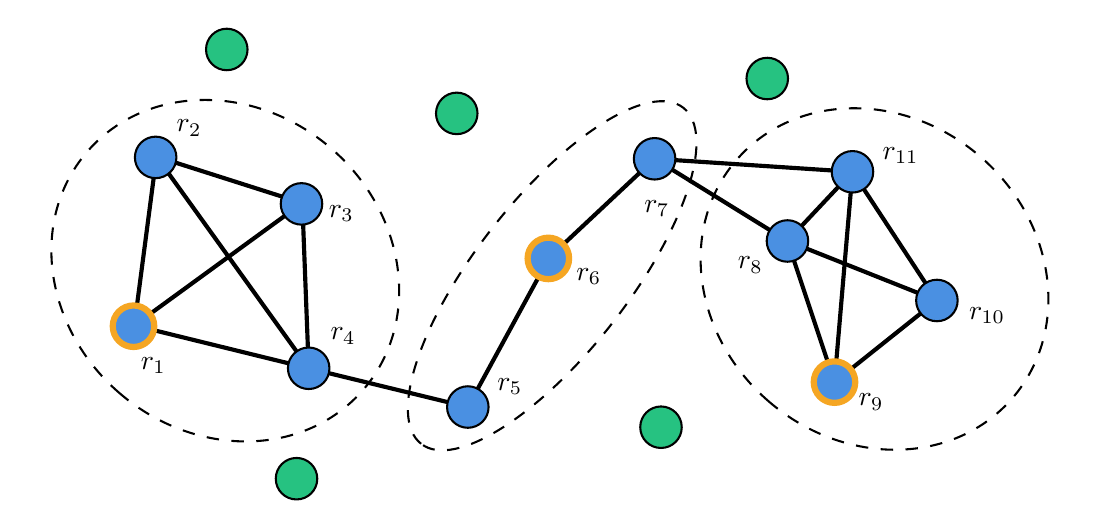
\begin{tikzpicture}[x=0.75pt,y=0.75pt,yscale=-1,xscale=1]
%uncomment if require: \path (0,300); %set diagram left start at 0, and has height of 300

%Straight Lines [id:da821267233332613] 
\draw [line width=1.5]    (122,74.33) -- (111.33,155.67) ;
%Straight Lines [id:da30341458803905486] 
\draw [line width=1.5]    (192.27,96.73) -- (122,74.33) ;
%Straight Lines [id:da15308567646882731] 
\draw [line width=1.5]    (192.27,96.73) -- (111.33,155.67) ;
%Straight Lines [id:da8895692654604979] 
\draw [line width=1.5]    (195.33,176.33) -- (111.33,155.67) ;
%Straight Lines [id:da8452110592323836] 
\draw [line width=1.5]    (195.33,176.33) -- (122,74.33) ;
%Straight Lines [id:da0975036779101448] 
\draw [line width=1.5]    (195.33,176.33) -- (192.27,96.73) ;
%Straight Lines [id:da6708709230251428] 
\draw [line width=1.5]    (426,115) -- (457.33,81.67) ;
%Straight Lines [id:da888005791791295] 
\draw [line width=1.5]    (448.67,183) -- (498,143.67) ;
%Straight Lines [id:da336628623261488] 
\draw [line width=1.5]    (448.67,183) -- (426,115) ;
%Straight Lines [id:da4856371467801972] 
\draw [line width=1.5]    (498,143.67) -- (457.33,81.67) ;
%Straight Lines [id:da9180518393029332] 
\draw [line width=1.5]    (498,143.67) -- (426,115) ;
%Straight Lines [id:da8952427329272475] 
\draw [line width=1.5]    (448.67,183) -- (457.33,81.67) ;
%Straight Lines [id:da8036283886157122] 
\draw [line width=1.5]    (272,195) -- (195.33,176.33) ;
%Straight Lines [id:da5584979597450603] 
\draw [line width=1.5]    (272,195) -- (311.2,123) ;
%Straight Lines [id:da816703332184367] 
\draw [line width=1.5]    (311.2,123) -- (362,75.4) ;
%Straight Lines [id:da907029535911398] 
\draw [line width=1.5]    (362,75.4) -- (457.33,81.67) ;
%Straight Lines [id:da5919582697274625] 
\draw [line width=1.5]    (362,75.4) -- (426,115) ;
%Shape: Circle [id:dp347326930362014] 
\draw  [fill={rgb, 255:red, 74; green, 144; blue, 226 }  ,fill opacity=1 ] (111.6,74.73) .. controls (111.6,69.21) and (116.08,64.73) .. (121.6,64.73) .. controls (127.12,64.73) and (131.6,69.21) .. (131.6,74.73) .. controls (131.6,80.26) and (127.12,84.73) .. (121.6,84.73) .. controls (116.08,84.73) and (111.6,80.26) .. (111.6,74.73) -- cycle ;
%Shape: Circle [id:dp9802636371346682] 
\draw  [fill={rgb, 255:red, 74; green, 144; blue, 226 }  ,fill opacity=1 ] (185.33,176.33) .. controls (185.33,170.81) and (189.81,166.33) .. (195.33,166.33) .. controls (200.86,166.33) and (205.33,170.81) .. (205.33,176.33) .. controls (205.33,181.86) and (200.86,186.33) .. (195.33,186.33) .. controls (189.81,186.33) and (185.33,181.86) .. (185.33,176.33) -- cycle ;
%Shape: Circle [id:dp48904188057709364] 
\draw  [color={rgb, 255:red, 245; green, 166; blue, 35 }  ,draw opacity=1 ][fill={rgb, 255:red, 74; green, 144; blue, 226 }  ,fill opacity=1 ][line width=2.25]  (100.93,156.07) .. controls (100.93,150.54) and (105.41,146.07) .. (110.93,146.07) .. controls (116.46,146.07) and (120.93,150.54) .. (120.93,156.07) .. controls (120.93,161.59) and (116.46,166.07) .. (110.93,166.07) .. controls (105.41,166.07) and (100.93,161.59) .. (100.93,156.07) -- cycle ;
%Shape: Circle [id:dp973523892724249] 
\draw  [fill={rgb, 255:red, 74; green, 144; blue, 226 }  ,fill opacity=1 ] (181.87,97.13) .. controls (181.87,91.61) and (186.34,87.13) .. (191.87,87.13) .. controls (197.39,87.13) and (201.87,91.61) .. (201.87,97.13) .. controls (201.87,102.66) and (197.39,107.13) .. (191.87,107.13) .. controls (186.34,107.13) and (181.87,102.66) .. (181.87,97.13) -- cycle ;
%Shape: Circle [id:dp5060420763706514] 
\draw  [fill={rgb, 255:red, 74; green, 144; blue, 226 }  ,fill opacity=1 ] (447.33,81.67) .. controls (447.33,76.14) and (451.81,71.67) .. (457.33,71.67) .. controls (462.86,71.67) and (467.33,76.14) .. (467.33,81.67) .. controls (467.33,87.19) and (462.86,91.67) .. (457.33,91.67) .. controls (451.81,91.67) and (447.33,87.19) .. (447.33,81.67) -- cycle ;
%Shape: Circle [id:dp8643742073771314] 
\draw  [fill={rgb, 255:red, 74; green, 144; blue, 226 }  ,fill opacity=1 ] (488,143.67) .. controls (488,138.14) and (492.48,133.67) .. (498,133.67) .. controls (503.52,133.67) and (508,138.14) .. (508,143.67) .. controls (508,149.19) and (503.52,153.67) .. (498,153.67) .. controls (492.48,153.67) and (488,149.19) .. (488,143.67) -- cycle ;
%Shape: Circle [id:dp32518754630200464] 
\draw  [fill={rgb, 255:red, 74; green, 144; blue, 226 }  ,fill opacity=1 ] (416,115) .. controls (416,109.48) and (420.48,105) .. (426,105) .. controls (431.52,105) and (436,109.48) .. (436,115) .. controls (436,120.52) and (431.52,125) .. (426,125) .. controls (420.48,125) and (416,120.52) .. (416,115) -- cycle ;
%Shape: Circle [id:dp1004066872083681] 
\draw  [color={rgb, 255:red, 245; green, 166; blue, 35 }  ,draw opacity=1 ][fill={rgb, 255:red, 74; green, 144; blue, 226 }  ,fill opacity=1 ][line width=2.25]  (438.67,183) .. controls (438.67,177.48) and (443.14,173) .. (448.67,173) .. controls (454.19,173) and (458.67,177.48) .. (458.67,183) .. controls (458.67,188.52) and (454.19,193) .. (448.67,193) .. controls (443.14,193) and (438.67,188.52) .. (438.67,183) -- cycle ;
%Shape: Circle [id:dp13679157078018644] 
\draw  [fill={rgb, 255:red, 74; green, 144; blue, 226 }  ,fill opacity=1 ] (262,195) .. controls (262,189.48) and (266.48,185) .. (272,185) .. controls (277.52,185) and (282,189.48) .. (282,195) .. controls (282,200.52) and (277.52,205) .. (272,205) .. controls (266.48,205) and (262,200.52) .. (262,195) -- cycle ;
%Shape: Circle [id:dp6424299525506494] 
\draw  [color={rgb, 255:red, 245; green, 166; blue, 35 }  ,draw opacity=1 ][fill={rgb, 255:red, 74; green, 144; blue, 226 }  ,fill opacity=1 ][line width=2.25]  (300.8,123.4) .. controls (300.8,117.88) and (305.28,113.4) .. (310.8,113.4) .. controls (316.32,113.4) and (320.8,117.88) .. (320.8,123.4) .. controls (320.8,128.92) and (316.32,133.4) .. (310.8,133.4) .. controls (305.28,133.4) and (300.8,128.92) .. (300.8,123.4) -- cycle ;

%Shape: Circle [id:dp3408789117010794] 
\draw  [fill={rgb, 255:red, 74; green, 144; blue, 226 }  ,fill opacity=1 ] (352,75.4) .. controls (352,69.88) and (356.48,65.4) .. (362,65.4) .. controls (367.52,65.4) and (372,69.88) .. (372,75.4) .. controls (372,80.92) and (367.52,85.4) .. (362,85.4) .. controls (356.48,85.4) and (352,80.92) .. (352,75.4) -- cycle ;
%Shape: Ellipse [id:dp9780793680593792] 
\draw  [dash pattern={on 4.5pt off 4.5pt}] (249.5,212.72) .. controls (233.44,200.19) and (248.69,153.79) .. (283.56,109.07) .. controls (318.43,64.36) and (359.72,38.26) .. (375.78,50.79) .. controls (391.84,63.31) and (376.59,109.72) .. (341.72,154.43) .. controls (306.85,199.15) and (265.56,225.24) .. (249.5,212.72) -- cycle ;
%Shape: Ellipse [id:dp17464640664522002] 
\draw  [dash pattern={on 4.5pt off 4.5pt}] (104.43,188.51) .. controls (67.6,156.96) and (60.44,104.88) .. (88.44,72.19) .. controls (116.44,39.5) and (169,38.57) .. (205.84,70.11) .. controls (242.67,101.66) and (249.83,153.74) .. (221.83,186.43) .. controls (193.82,219.13) and (141.26,220.06) .. (104.43,188.51) -- cycle ;
%Shape: Ellipse [id:dp7547054439217645] 
\draw  [dash pattern={on 4.5pt off 4.5pt}] (417.23,192.51) .. controls (380.4,160.96) and (373.24,108.88) .. (401.24,76.19) .. controls (429.24,43.5) and (481.8,42.57) .. (518.64,74.11) .. controls (555.47,105.66) and (562.63,157.74) .. (534.63,190.43) .. controls (506.62,223.13) and (454.06,224.06) .. (417.23,192.51) -- cycle ;
%Shape: Circle [id:dp07179305757060428] 
\draw  [fill={rgb, 255:red, 38; green, 194; blue, 129 }  ,fill opacity=1 ] (256.67,53.53) .. controls (256.67,48.01) and (261.14,43.53) .. (266.67,43.53) .. controls (272.19,43.53) and (276.67,48.01) .. (276.67,53.53) .. controls (276.67,59.06) and (272.19,63.53) .. (266.67,63.53) .. controls (261.14,63.53) and (256.67,59.06) .. (256.67,53.53) -- cycle ;
%Shape: Circle [id:dp6276221659819717] 
\draw  [fill={rgb, 255:red, 38; green, 194; blue, 129 }  ,fill opacity=1 ] (355.07,204.73) .. controls (355.07,199.21) and (359.54,194.73) .. (365.07,194.73) .. controls (370.59,194.73) and (375.07,199.21) .. (375.07,204.73) .. controls (375.07,210.26) and (370.59,214.73) .. (365.07,214.73) .. controls (359.54,214.73) and (355.07,210.26) .. (355.07,204.73) -- cycle ;
%Shape: Circle [id:dp8257521060147176] 
\draw  [fill={rgb, 255:red, 38; green, 194; blue, 129 }  ,fill opacity=1 ] (179.47,229.53) .. controls (179.47,224.01) and (183.94,219.53) .. (189.47,219.53) .. controls (194.99,219.53) and (199.47,224.01) .. (199.47,229.53) .. controls (199.47,235.06) and (194.99,239.53) .. (189.47,239.53) .. controls (183.94,239.53) and (179.47,235.06) .. (179.47,229.53) -- cycle ;
%Shape: Circle [id:dp5988037975306492] 
\draw  [fill={rgb, 255:red, 38; green, 194; blue, 129 }  ,fill opacity=1 ] (145.87,22.73) .. controls (145.87,17.21) and (150.34,12.73) .. (155.87,12.73) .. controls (161.39,12.73) and (165.87,17.21) .. (165.87,22.73) .. controls (165.87,28.26) and (161.39,32.73) .. (155.87,32.73) .. controls (150.34,32.73) and (145.87,28.26) .. (145.87,22.73) -- cycle ;
%Shape: Circle [id:dp013478726522430984] 
\draw  [fill={rgb, 255:red, 38; green, 194; blue, 129 }  ,fill opacity=1 ] (406.27,36.73) .. controls (406.27,31.21) and (410.74,26.73) .. (416.27,26.73) .. controls (421.79,26.73) and (426.27,31.21) .. (426.27,36.73) .. controls (426.27,42.26) and (421.79,46.73) .. (416.27,46.73) .. controls (410.74,46.73) and (406.27,42.26) .. (406.27,36.73) -- cycle ;

% Text Node
\draw (112.93,169.47) node [anchor=north west][inner sep=0.75pt]    {$r_{1}$};
% Text Node
\draw (130.2,55.2) node [anchor=north west][inner sep=0.75pt]    {$r_{2}$};
% Text Node
\draw (203.6,96.4) node [anchor=north west][inner sep=0.75pt]    {$r_{3}$};
% Text Node
\draw (204.4,155.4) node [anchor=north west][inner sep=0.75pt]    {$r_{4}$};
% Text Node
\draw (284.8,179.6) node [anchor=north west][inner sep=0.75pt]    {$r_{5}$};
% Text Node
\draw (322.8,126.8) node [anchor=north west][inner sep=0.75pt]    {$r_{6}$};
% Text Node
\draw (355.6,94) node [anchor=north west][inner sep=0.75pt]    {$r_{7}$};
% Text Node
\draw (400.6,121.2) node [anchor=north west][inner sep=0.75pt]    {$r_{8}$};
% Text Node
\draw (458.8,187.2) node [anchor=north west][inner sep=0.75pt]    {$r_{9}$};
% Text Node
\draw (512,145.6) node [anchor=north west][inner sep=0.75pt]    {$r_{10}$};
% Text Node
\draw (470.4,68.4) node [anchor=north west][inner sep=0.75pt]    {$r_{11}$};


\end{tikzpicture}


	\caption[Dynamic Groups]{An illustration showing the dynamic nature of groups. Here we have blue and green robots, where every blue robot only trusts other blue robots. A line between the pair of robots $r_i$ and $r_j$ indicates that they can observe one another. Robots with a golden outline are leaders, whilst the others are followers. We see that $r_1$ can observe  $r_2$, $r_3$ and $r_4$. Similarly, $r_6$ can observe $r_5$ and $r_7$ and $r_9$ can observe $r_8$, $r_{10}$ and $r_{11}$}
 \label{fig:dyn_group}
\end{figure}


\subsubsection{Leaders}
Leaders act as anchors for the group; providing a good approximation of followers' ground truth poses. In order to do this, they must first have a high-quality localisation. This is guaranteed as leaders are strongly-defended. At each iteration of the RobotWeb, a leader will reject all messages it receives, unless they were sent by a fellow leader in the same group. As we later prove in \autoref{section:proof-correctness}, this provides a strong defence for leaders. A leader will also send messages to its followers, about its belief about their localisations. The leader will indicate that the messages are from a leader by setting a ``leader flag''.

\RestyleAlgo{ruled}

%% This is needed if you want to add comments in
%% your algorithm with \Comment
\SetKwComment{Comment}{/* }{ */}

\begin{algorithm}[H]
\DontPrintSemicolon
\caption{Leader Message Filter}\label{alg:leader-msg-filter}
\SetKwFunction{origin}{origin}
\SetKwFunction{group}{group}
\SetKwFunction{role}{role}
\SetKwData{leader}{LEADER}
\SetKw{And}{and}


\KwIn{A set of incoming messages $M = \{m_1, m_2, \dots, m_3\}$}
\KwOut{The filtered set of messages $F = \{f_1, f_2, \dots, f_3\}$}

\BlankLine
\ForEach{message $m_i$ of $M$}{
\If{\group{\origin{$m_i$}} = \group{this} \And \role{$m_1$} = \leader}{
        $F \overset{+}{\leftarrow} m_i$\;
    }
 }
\end{algorithm}

\subsubsection{Followers}
Followers instead act as bridges between the group and the wider RobotWeb, using it to refine their localisations. At every iteration of the RobotWeb, a follower will receive a set of messages. First, it will combine all the leaders' messages (indicated by the ``leader flag'') to form a baseline estimate of its ground truth pose. It will then use this estimate to reject all other messages if the distance between their claimed pose, and the estimate is greater than the configurable parameter $\epsilon$. As we later prove in \autoref{section:proof-correctness}, this provides a weak defence for followers. 

In some cases, the messages sent by leaders may not provide information about every aspect of the follower's localisation. For example, a follower drone may only receive information about its position in three-dimensional space, and nothing about its bearing. In this case, the follower will ignore all messages which make claims about its bearing, as does not possess a means by which to verify these claims. 

\begin{algorithm}[H]
\DontPrintSemicolon
\caption{Follower Message Filter}\label{alg:follower-msg-filter}
\SetKwFunction{origin}{origin}
\SetKwFunction{group}{group}
\SetKwFunction{role}{role}
\SetKwData{leader}{LEADER}
\SetKw{Continue}{continue}
\SetKw{And}{and}
\SetKw{Or}{or}

\KwIn{A set of incoming messages $M = \{m_1, m_2, \dots, m_3\}$}
\KwOut{The filtered set of messages $F = \{f_1, f_2, \dots, f_3\}$}
\BlankLine
\tcp{Constructing the Baseline Estimate}
$\eta_l \leftarrow \mathbf{0}$\; 
$\Lambda_l \leftarrow \mathbf{0}$\; 
\ForEach{message $m_i = \left(\eta_i, \Lambda_i\right)$ of $M$}{
    \If{\group{\origin{$m_i$}} = \group{this} \And \role{$m_1$} = \leader}{
            $\eta_l \leftarrow \eta_l + \eta_i$\; 
            $\Lambda_l \leftarrow \Lambda_l + \Lambda_i$\; 
    }
 }
 
 $\mu_l \leftarrow \Lambda_l^{-1} \eta_l$ \tcp{Baseline Estimate}
 
\BlankLine
\tcp{Filtering out messages}
 \ForEach{message $m_i = \left(\eta_i, \Lambda_i\right)$ of $M$}{
    \If{\group{\origin{$m_i$}} $\neq$ \group{this} \Or \role{$m_1$} $\neq$ \leader}{
            $\mu_i \leftarrow \Lambda_i^{-1}\eta_i$\;
            \If{$\norm{\mu_i - \mu_l} > \epsilon$}{
                \Continue\;
            }
    }
    $F \overset{+}{\leftarrow} m_i$\;
 }

\end{algorithm}

\subsubsection{Group Formation} \label{section:group-formation}
Now we have seen which roles are present within a group, and their respective purposes, we will discuss how groups form, and how each robot initially decides its role.

Initially, a robot will assume the role of a follower, so it can benefit from any nearby leaders. However, these leaders are not guaranteed to be present. Let us now consider a scenario where a group consists only of followers - this group will be unprotected. This will prompt each member to assume leadership, to put them \textit{under its aegis}. However, this behaviour will lead to a thundering herd of robots, all clamouring to assume leadership, and thus producing a group that consists only of leaders. This situation is also far from ideal, as although the group is protected, it has no bridges to the wider RobotWeb.

We aim to mitigate this problem by introducing randomised timers, inspired by the Raft consensus algorithm \cite{raft}. Now, when a follower detects a lack of leaders, it will wait for a random, but bounded, amount of time before assuming leadership. While it waits, the follower will ignore all messages it receives, regardless of their origins. If while it is waiting, the robot detects that a sufficient number of leaders ($\geq L_{min}$) exists, it will cancel its timer and return to operating as a follower.

So far, this solution only mitigates the problem, instead of solving it as there is a small but non-zero chance that all robots' timers fire simultaneously. If this were to happen, then the group would once again consist solely of leaders. We further mitigate this problem by introducing a second randomised timer, but instead for leaders. Now if a leader detects a surplus of leaders ($> L_{max}$), it will start this timer. When the timer fires, the leader will resign. Once again, the leader will cancel its timer if it stops detecting this surplus.

Together, the combination of these two timers will ensure that the group will eventually contain a good balance of leaders and followers.

\subsubsection{Role Changes}
Eventually, a leader will seek to become a follower regardless of the number of leaders in the group. The reason for this is twofold: by ignoring messages from non-leaders, leaders trade the benefits of participating in the wider RobotWeb for security guarantees. This means that the longer a leader serves, the worse the quality of its localisation is likely to be, compared to its followers. In order to maintain fairness, we introduce a \textbf{succession} mechanism, which allows leaders to retire and appoint a successor.

\begin{figure}[!h]
	\centering
	

\tikzset{every picture/.style={line width=0.75pt}} %set default line width to 0.75pt        

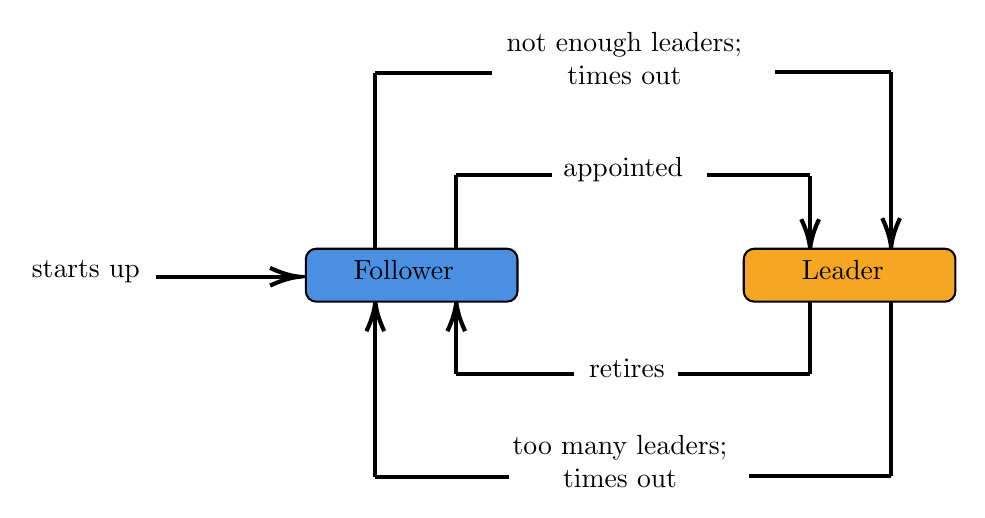
\begin{tikzpicture}[x=0.75pt,y=0.75pt,yscale=-1,xscale=1]
%uncomment if require: \path (0,300); %set diagram left start at 0, and has height of 300

%Straight Lines [id:da7582024624443486] 
\draw [line width=1.5]    (74.5,153.75) -- (140.5,153.75) ;
\draw [shift={(143.5,153.75)}, rotate = 180] [color={rgb, 255:red, 0; green, 0; blue, 0 }  ][line width=1.5]    (14.21,-4.28) .. controls (9.04,-1.82) and (4.3,-0.39) .. (0,0) .. controls (4.3,0.39) and (9.04,1.82) .. (14.21,4.28)   ;
%Straight Lines [id:da1737175708146408] 
\draw [line width=1.5]    (219,168.75) -- (219,200.75) ;
\draw [shift={(219,165.75)}, rotate = 90] [color={rgb, 255:red, 0; green, 0; blue, 0 }  ][line width=1.5]    (14.21,-4.28) .. controls (9.04,-1.82) and (4.3,-0.39) .. (0,0) .. controls (4.3,0.39) and (9.04,1.82) .. (14.21,4.28)   ;
%Straight Lines [id:da0069991711386795386] 
\draw [line width=1.5]    (180,168.75) -- (180,250.25) ;
\draw [shift={(180,165.75)}, rotate = 90] [color={rgb, 255:red, 0; green, 0; blue, 0 }  ][line width=1.5]    (14.21,-4.28) .. controls (9.04,-1.82) and (4.3,-0.39) .. (0,0) .. controls (4.3,0.39) and (9.04,1.82) .. (14.21,4.28)   ;
%Straight Lines [id:da7997009254563132] 
\draw [line width=1.5]    (219,104.75) -- (219,139.75) ;
%Straight Lines [id:da6517634793539615] 
\draw [line width=1.5]    (180,55.75) -- (180,140.25) ;
%Straight Lines [id:da9381133415973326] 
\draw [line width=1.5]    (389.5,137.25) -- (389.5,105.25) ;
\draw [shift={(389.5,140.25)}, rotate = 270] [color={rgb, 255:red, 0; green, 0; blue, 0 }  ][line width=1.5]    (14.21,-4.28) .. controls (9.04,-1.82) and (4.3,-0.39) .. (0,0) .. controls (4.3,0.39) and (9.04,1.82) .. (14.21,4.28)   ;
%Straight Lines [id:da20475050027342967] 
\draw [line width=1.5]    (428.5,136.75) -- (428.5,55.25) ;
\draw [shift={(428.5,139.75)}, rotate = 270] [color={rgb, 255:red, 0; green, 0; blue, 0 }  ][line width=1.5]    (14.21,-4.28) .. controls (9.04,-1.82) and (4.3,-0.39) .. (0,0) .. controls (4.3,0.39) and (9.04,1.82) .. (14.21,4.28)   ;
%Straight Lines [id:da6314202210947096] 
\draw [line width=1.5]    (389.5,200.75) -- (389.5,165.75) ;
%Straight Lines [id:da8469144916993987] 
\draw [line width=1.5]    (428.5,249.75) -- (428.5,165.25) ;
%Straight Lines [id:da6059987412847359] 
\draw [line width=1.5]    (219,104.75) -- (265,104.75) ;
%Straight Lines [id:da8345372265263031] 
\draw [line width=1.5]    (340,104.75) -- (389.5,104.75) ;
%Straight Lines [id:da759250238348591] 
\draw [line width=1.5]    (219,200.75) -- (275.5,200.75) ;
%Straight Lines [id:da004199534393038551] 
\draw [line width=1.5]    (326,200.75) -- (389.5,200.75) ;
%Straight Lines [id:da6463360435279583] 
\draw [line width=1.5]    (180,55.75) -- (236,55.75) ;
%Straight Lines [id:da9478179483720361] 
\draw [line width=1.5]    (372.5,55.25) -- (428.5,55.25) ;
%Straight Lines [id:da38872862853815515] 
\draw [line width=1.5]    (360,249.75) -- (428.5,249.75) ;
%Straight Lines [id:da9605862890532954] 
\draw [line width=1.5]    (180,250.25) -- (244.5,250.25) ;
%Rounded Rect [id:dp1761614463331822] 
\draw  [fill={rgb, 255:red, 74; green, 144; blue, 226 }  ,fill opacity=1 ] (146.5,145.35) .. controls (146.5,142.53) and (148.78,140.25) .. (151.6,140.25) -- (243.4,140.25) .. controls (246.22,140.25) and (248.5,142.53) .. (248.5,145.35) -- (248.5,160.65) .. controls (248.5,163.47) and (246.22,165.75) .. (243.4,165.75) -- (151.6,165.75) .. controls (148.78,165.75) and (146.5,163.47) .. (146.5,160.65) -- cycle ;

%Rounded Rect [id:dp11855608762791614] 
\draw  [fill={rgb, 255:red, 245; green, 166; blue, 35 }  ,fill opacity=1 ] (357.5,145.35) .. controls (357.5,142.53) and (359.78,140.25) .. (362.6,140.25) -- (454.4,140.25) .. controls (457.22,140.25) and (459.5,142.53) .. (459.5,145.35) -- (459.5,160.65) .. controls (459.5,163.47) and (457.22,165.75) .. (454.4,165.75) -- (362.6,165.75) .. controls (359.78,165.75) and (357.5,163.47) .. (357.5,160.65) -- cycle ;


% Text Node
\draw (384,144.5) node [anchor=north west][inner sep=0.75pt]   [align=left] {Leader};
% Text Node
\draw (168,144.5) node [anchor=north west][inner sep=0.75pt]   [align=left] {Follower};
% Text Node
\draw (13,144.5) node [anchor=north west][inner sep=0.75pt]   [align=left] {starts up};
% Text Node
\draw (236.5,34.25) node [anchor=north west][inner sep=0.75pt]   [align=left] {\begin{minipage}[lt]{92.96pt}\setlength\topsep{0pt}
\begin{center}
not enough leaders;\\times out
\end{center}

\end{minipage}};
% Text Node
\draw (269,94.5) node [anchor=north west][inner sep=0.75pt]   [align=left] {appointed};
% Text Node
\draw (279,192) node [anchor=north west][inner sep=0.75pt]   [align=left] {\begin{minipage}[lt]{31.08pt}\setlength\topsep{0pt}
\begin{center}
retires
\end{center}

\end{minipage}};
% Text Node
\draw (240.5,228.75) node [anchor=north west][inner sep=0.75pt]   [align=left] {\begin{minipage}[lt]{83.84pt}\setlength\topsep{0pt}
\begin{center}
too many leaders;\\times out
\end{center}

\end{minipage}};


\end{tikzpicture}


    \caption[Role Change State Machine]{The rules for role changes. A follower becomes a leader when it is appointed by a leader, or when it assumes leadership as too few leaders are present. A leader becomes a follower when it retires or when too many leaders are present.}
\end{figure}

There are two questions that guide the design of this mechanism:
\begin{enumerate*}
    \item ``When should a leader retire?'' and
    \item ``Which robot should it appoint as its successor?''.
\end{enumerate*}
We codify the answers to these questions as the \textbf{Retirement Policy} and the \textbf{Successor Identification Policy}.

An effective Retirement Policy would have a leader serve the optimal term length. Ideally, this means that a leader serves for as long as possible and no longer. If a leader's tenure is too long, then the quality of its localisation may degrade, and so would the quality of its ground truth pose estimates. Yet, if a leader's tenure is too short, then it will introduce needless role changes, which the rest of the group would need to handle, needlessly consuming extra computational resources.

An effective Successor Identification Policy would result in the appointment of the most suitable follower as a successor. One follower is more suitable than another if it can \begin{enumerate}
    \item Serve for more time.
    \item Provide better ground truth pose estimates.
    \item Serve more followers.
\end{enumerate}
However, designing a policy that achieves these goals is complicated, since each goal can be affected by many factors. For example, a follower with a higher quality localisation may serve for less time than another with a lower quality one, if it moves away from its followers.

After a leader has chosen a good successor, it would inform its successor about the change and subsequently resign. However, the successor cannot immediately assume leadership, as it could weaken the defences of the group. Successors are weakly-defended, meaning that they could be subtly biased. If then a biased successor were to be appointed leader, then that leader would itself be biased. Through contagion, this bias would slowly spread throughout the group. We prevent this problem by introducing a \textbf{transitory step} for successors. Before a successor can assume leadership, it must first reset its past localisations, to its leaders' beliefs. This ensures that the new leader is unbiased. 

\subsubsection{Exits, Mergers, and Acquisitions}
In Aegis, there are three important events that can occur. They are exits (when a robot leaves a group), mergers (when multiple mutually trusted groups encounter one another), and acquisitions (when a robot encounters a group that it trusts). We will now briefly discuss how the group will react to each of these events.

A robot may exit its group at any time. This may happen when the robot has physically moved away from the group and so cannot sense any of them, or it may happen if the robot suffers an internal fault. Regardless of the reason behind an exit, the group is largely unaffected. If the exiting robot is a leader, then it should instead appoint a successor before it leaves. Although this is not necessary, since the group will soon replace it. If instead, the exiting robot is a follower, then the group does not need to take action, since followers do not directly affect the group. After exiting, the follower would eventually observe that it has no leaders and appoint itself leader.

When multiple groups of robots merge, no action will be taken at first. Instead, the robots in the merged group would recognise that there are more leaders than needed. This would prompt some of the extraneous leaders to resign, thus restoring a healthy balance between leaders and followers.

In most circumstances where a group acquires a robot, the robot will be a leader, since individual robots can be thought of as ``groups of 1''. Since leaders are strongly-defended, the group does not need to directly take action. If acquiring a leader results in a surplus of leaders, then an extraneous leader will resign. There is one scenario where a group can acquire a follower, which is if the robot has just joined the RobotWeb. Here no action needs to be taken.

\subsection{A Proof of Correctness} \label{section:proof-correctness}
We will now formally prove the correctness of Aegis. It is correct if and only if \begin{enumerate*}
    \item leaders are strongly-defended, 
    \item followers are weakly-defended and
    \item the transitory step transforms a weakly-defended robot into a strongly-defended one.
\end{enumerate*}
\subsubsection{Leaders}
We consider a situation where the set of robots, $R$, is covered by the set of groups $GS$ and the set of attackers $A$, such that every robot in $R$ either belongs to a single group $G_i \in GS$ or is an attacker. Every group $G_i$ is covered by $L_i \cup F_i$ which refers to the leaders and followers in the group respectively. Since solitary robots act as leaders of groups of 1, $|F_i| = 1$.

At each iteration of the RobotWeb, a robot $r_i$ may send a message, $m_{ij}$ to $r_j$, where $m_{ij} := (\mu_{ij}, \Sigma_{ij}) = (\Lambda_{ij}^{-1}\eta_{ij}, \Lambda_{ij}^{-1})$.

We also define the following predicates:
\begin{align*}
    \mathbf{leader(r_i)} &\triangleq \exists{G_k \in GS}\left[r_i \in G_k \land r_i \in L_k\right]\\
    \mathbf{follower(r_i)} &\triangleq \exists{G_k \in GS}\left[r_i \in G_k \land r_i \in F_k\right]\\
    \mathbf{trusts(r_i, r_j)} &\triangleq leader(r_i) \implies (\exists{G \in GS}\left[r_i \in G \land r_j \in G\right] \land leader(r_j))\\
    \mathbf{accepts(r_i, m_{jk})} &\triangleq trusts(r_i, r_j)\\
    \mathbf{victim(r_i, r_a)} &\triangleq trusts(r_i, r_a) \lor \exists r_j \in R\left[trusts(r_i, r_j) \land victim(r_j, r_a)\right]
\end{align*}

Now in order to prove that leaders are \textbf{strongly-defended}, we must show that the following cannot hold:
\begin{equation}
    \exists r_i\in R, r_a \in A\left[leader(r_i) \land victim(r_i, r_a)\right]
\end{equation}
We take an arbitrary $r_i \in R$ and $r_a \in A$, such that $leader(r_i)$ holds. Now it is sufficient for us to prove that $victim(r_i, r_a)$ cannot hold.
\begin{align*}
    victim(r_i, r_a) \iff trusts(r_i, r_a) \lor \exists r_j \in R\left[trusts(r_i, r_j) \land victim(r_j, r_a)\right]
\end{align*}

First, we prove the left hand side cannot hold.
\begin{align*}
    trusts(r_i, r_a) &\iff leader(r_i) \implies (\exists{G \in GS}\left[r_i \in G \land r_a \in G\right] \land leader(r_a)) \tag*{\text{By the definition of trusts($r_i$, $r_j$)}}\\
    &\iff \exists{G \in GS}\left[r_i \in G \land r_a \in G\right] \land leader(r_a) \tag*{\text{By the assumption that leader($r_i$) holds}}\\\
    &\iff False \land False \tag*{\text{Since $\neg \exists G\in GS\left[r_a\in G\right]$}}\\
    &\iff False
\end{align*}

Then we prove that the right hand side also cannot hold, by taking an arbitrary $r_j \in R$. Since $trusts(r_i, r_j)$ must hold, $r_j$ must be a leader in the same group as $r_i$. However, now as $r_j$ is a leader and a victim of $r_a$, there must exist some other robot $r_k \in R$ that $r_j$ trusts and is a victim of $r_a$. Since $r_j$ trusts $r_k$, it must be another leader in the same group as $r_i$ and $r_j$, and so yet another robot $r_l$ must exist, that is trusted by $r_k$ and is a victim of $r_a$. This recursion continues ad infinitum, but since the number of leaders in a group is finite, this cannot be possible. Hence the right hand side also doesn't hold.

Since neither the left nor right hand sides hold, $victim(r_i, r_a)$ also cannot hold. Thus it is impossible for an attacker to influence a leader, and so leaders are well-defended.
\subsubsection{Followers}
Unlike leaders, followers can be influenced by attackers as they accept messages from all robots. Yet we can still prove that they are well-defended by proving that they will localise to points close to the ground truth, instead of the arbitrary points suggested by attackers. 

At each iteration of belief propagation, a follower will receive a set of messages $M$. These can be grouped into 2 distinct sets consisting of messages from its leaders, $M_l$, and other robots in the RobotWeb, $M_r$), where a subset, $M_a \subseteq M_r$, will be sent by attackers. The robot will first use \autoref{eqn:gbp-sum} to combine the leaders' messages into the baseline estimate, $N(\mu_l, \Sigma_l)$. Then it will measure the distance between each message $m_i \in M_r$ from $\mu_l$ and filter out any message $m_i = (\mu_i, \Sigma_i)$ where $||\mu_i - \mu_l||_2 > \epsilon$. Finally, it will combine all messages that passed through the filter and the leaders' messages, using \autoref{eqn:gbp-sum}, to compute its final belief, $(\mu, \Sigma)$. For an attack to be successful, the final belief must escape the $\epsilon$-bound, otherwise, the follower's localisation will always closely follow its ground truth pose. Formally, this means:

\begin{theorem}[Criteria for a Successful Attack]
\label{theo:successful-attack-criteria}
An attack can be considered to be successful if and only if there exists $M_a$ such that the final localisation $\mu$ of the attacked robot satisfies: \[\norm{\mu - \mu_l} > \epsilon \tag{where $\epsilon > 0$}\]
\end{theorem}

We will now prove that \ref{theo:successful-attack-criteria} cannot be satisfied.

Let $M_c$ represent the union between all the messages passed through the filter and the leaders' messages. We know that the following holds:
\begin{equation}
    \forall i \in M_c \left[ \norm{\mu_i - \mu_l} \leq \epsilon\right] \label{eqn:all_smaller}
\end{equation}

The Euclidean distance between the final localisation and the baseline estimate is:
\begin{align}
    \norm{\mu - \mu_l} &= \norm{\left(\sum_{i \in M_c} \left(\sum_{j \in M_c} \Lambda_j\right)^{-1} \eta_i\right)  - \mu_l} \tag*{\text{By \ref{eqn:gbp-sum}}}\\
    &= \norm{\left(\sum_{i \in M_c} \left(\sum_{j \in M_c} \Lambda_j\right)^{-1} \Lambda_i\mu_i\right)  - \mu_l} \tag*{\text{By \ref{eqn:canonical}}}
\end{align}

Now noticing that:
\begin{align}
    I &= A^{-1}A\\
      &= \left(\sum_{i \in M_c} \Lambda_i\right)^{-1}\left(\sum_{i \in M_c} \Lambda_i\right)\\
      &= \sum_{i \in M_c} \left(\sum_{j \in M_c} \Lambda_j\right)^{-1}\Lambda_i \label{eqn:sub}
\end{align}
We can substitute \autoref{eqn:sub} into the above expression for the Euclidean distance between the final localisation and baseline estimate to obtain:
\begin{align}
    \norm{\mu - \mu_l} &= \norm{\left(\sum_{i \in M_c} \left(\sum_{j \in M_c} \Lambda_j\right)^{-1} \Lambda_i\mu_i\right)  - I\mu_l}\\
    &= \norm{\left(\sum_{i \in M_c} \left(\sum_{j \in M_c} \Lambda_j\right)^{-1} \Lambda_i\mu_i\right)  - \left(\sum_{i \in M_c} \left(\sum_{j \in M_c} \Lambda_j\right)^{-1}\Lambda_i\right)\mu_l}\\
     &= \norm{\sum_{i \in M_c} \left(\sum_{j \in M_c} \Lambda_j\right)^{-1} \Lambda_i\left(\mu_i - \mu_l\right)}\\
     &\leq \sum_{i \in M_c} \norm{\left(\sum_{j \in M_c} \Lambda_j\right)^{-1} \Lambda_i\left(\mu_i - \mu_l\right)} \tag*{By the sub-additive property}\\
     &\leq \sum_{i \in M_c} \norm{\left(\sum_{j \in M_c} \Lambda_j\right)^{-1} \Lambda_i}\norm{\mu_i - \mu_l} \tag*{By the sub-multiplicative property}
\end{align}
Now that we have an upper bound on the distance, we can use \autoref{eqn:all_smaller} to simplify the second norm so we have:
\begin{align}
    \norm{\mu - \mu_l} &\leq \epsilon\sum_{i \in M_c} \norm{\left(\sum_{j \in M_c} \Lambda_j\right)^{-1} \Lambda_i}
\end{align}
So now it is sufficient to prove that:
\begin{align}
    \sum_{i \in M_c} \norm{\left(\sum_{j \in M_c} \Lambda_j\right)^{-1} \Lambda_i} \leq 1
\end{align}
To simplify the following equations we make the following substitution:
\begin{align}
    \Omega_i = \left(\sum_{j \in M_c} \Lambda_j\right)^{-1} \Lambda_i
\end{align}

As we are using the induced l2 matrix norm, the value of $\norm{A}$ for some matrix $A$ is equal to its largest singular value. If $A$ is a symmetric matrix, we can make a further simplification and say that $\norm{A} = \lambda_{max}(A)$ where $\lambda_{max}(A)$ is the largest eigenvalue of $A$.

The matrix $\Lambda_i$ is a precision matrix, and so is guaranteed to be symmetric positive definite. We know that the sums, inverses, and matrix products of symmetric positive definite matrices are also symmetric positive definite matrices, meaning that $\Omega_i$ is guaranteed to be symmetric positive definite.

So now $\norm{\Omega_i} = \lambda_{max}(\Omega_i)$, which allows us to use Weyl's Inequality about Perturbation \cite{weyls}, which gives us the following inequality:
\begin{equation}
    \lambda_{max}\left(\sum_{i \in M_c} \Omega_i\right) \leq \sum_{i \in M_c} \lambda_{max}(\Omega_i)
\end{equation}
And since $\Omega_i$ is positive definite, we can guarantee that each eigenvalue is greater than 0. This satisfies an equality condition derived in \cite{weyls_equality} allowing us to write:
\begin{align}
    \sum_{i \in M_c} \lambda_{max}(\Omega_i) &= \lambda_{max}\left(\sum_{i \in M_c} \Omega_i\right)\\
    &= \lambda_{max}(I) \tag*{\text{By \ref{eqn:sub}}}\\
    &= 1
\end{align}

Therefore:
\begin{align}
    \norm{\mu - \mu_l} &\leq \epsilon\sum_{i \in M_c} \norm{\left(\sum_{j \in M_c} \Lambda_j\right)^{-1} \Lambda_i}\\
    &= \epsilon \sum_{i \in M_c} \norm{\Omega_i}\\
    &= \epsilon
\end{align}

And thus \ref{theo:successful-attack-criteria} cannot hold.\\

\subsubsection{Transitory Step}
The transitory step forces a follower to reset its localisations to those suggested by its leaders. As we have seen before, attackers are unable to influence leaders' beliefs, and so cannot influence the follower's new localisations. This means that the follower is now strongly-defended.

\section{Evaluation} \label{section:eval-def}
Now we shall evaluate Aegis in the same simulated environment as before. Our goal here is to explore and understand how our solution performs. To do this, we will first perform three separate analyses to evaluate how well it performs when robots are under attack, when are no longer under attack, and when are not being attacked. 

\subsection{Experimental Setup}
Our experimental setup here shares many similarities with its predecessor in \autoref{section:attacker_experiments}. We still have a single attacker against $n$ normal robots. Our robots still move along and localise to predefined paths and our attackers still try to trick them into localising onto another path. Finally, we will use the same configurable parameters as detailed in \autoref{table:attack-expr-params}. We will also extend the robots' sensing range to cover the entire area, in order to keep a constant number of leaders throughout.

In addition to these parameters, we introduce several more aimed at configuring groups. They are listed below in \autoref{table:defence-expr-params}

%TODO: fix table
\begin{table}[!ht]
\centering
\resizebox{\textwidth}{!}{%
\begin{tabular}{|c|c|c|}
\hline
\textbf{Parameter}              & \textbf{Description}                                                                               & \textbf{Default Value} \\ \hline
Maximum Leader Divergence       & The maximum distance that an accepted message can be from the baseline estimate. & 0.01m                  \\ \hline
Leader Timeout                  & The maximum time that a robot can be leaderless without appointing itself as a leader.             & 5 ticks                \\ \hline
Minimum Leader Count            & The minimum number of leaders that a robot should observe.                                         & 1                      \\ \hline
Maximum Leader Count            & The maximum number of leaders that a robot should observe.                                         & 1                      \\ \hline
Retirement Policy               & The policy used by a leader to decide when it should retire.                                       & Random: $p = 0.1$                \\ \hline
Successor Identification Policy & The policy used by a leader to decide on a successor.                                              & Random                 \\ \hline
\end{tabular}%
}
\caption{The default parameters used to configure groups in these experiments}
\label{table:defence-expr-params}
\end{table}


\subsubsection{Path Design}
However, our current setup does also differ from its predecessor. Most notably, we choose to use more realistic paths. We consider a scenario where multiple robots are patrolling a miniaturised rainforest, to prevent illegal deforestation. If the robots notice any suspicious activity, they will alert the forest rangers of their locations, and the rangers will investigate. Now a logger who wishes to sabotage this system would attack the RobotWeb. Their attackers would try to distort the patrollers' localisations to keep the rangers from searching in a specific area. We present these paths in the below diagram. Note that we have shrunk the area of the rainforest down to a 1m by 1m grid, for ease of visualisation; in practice, this should not matter.

\begin{figure}[!h]
	\centering
	

\tikzset{every picture/.style={line width=0.75pt}} %set default line width to 0.75pt        

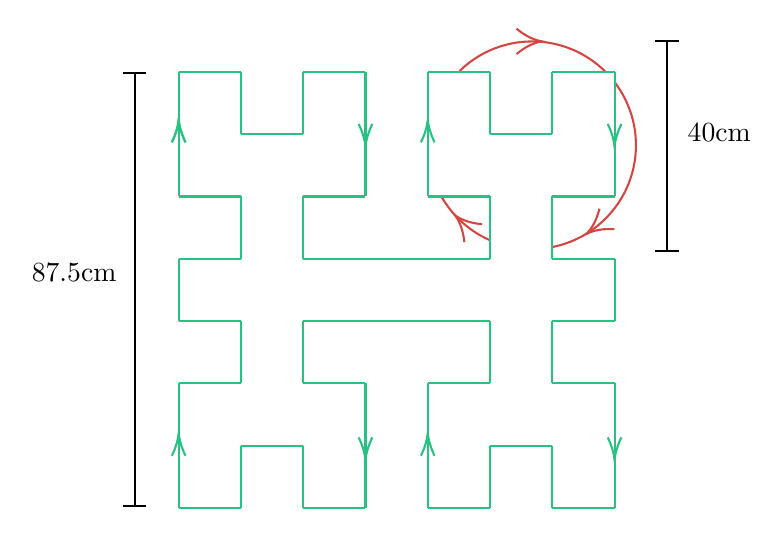
\begin{tikzpicture}[x=0.75pt,y=0.75pt,yscale=-1,xscale=1]
%uncomment if require: \path (0,300); %set diagram left start at 0, and has height of 300

%Shape: Arc [id:dp2186219161659576] 
\draw  [draw opacity=0] (380.97,43.57) .. controls (387.25,51.93) and (390.97,62.31) .. (390.97,73.57) .. controls (390.97,97.88) and (373.62,118.14) .. (350.62,122.64) -- (340.97,73.57) -- cycle ; \draw  [color={rgb, 255:red, 214; green, 69; blue, 65 }  ,draw opacity=1 ] (380.97,43.57) .. controls (387.25,51.93) and (390.97,62.31) .. (390.97,73.57) .. controls (390.97,97.88) and (373.62,118.14) .. (350.62,122.64) ;  
%Shape: Arc [id:dp14231683771998604] 
\draw  [draw opacity=0] (306.04,37.79) .. controls (315.05,28.99) and (327.38,23.57) .. (340.97,23.57) .. controls (354.86,23.57) and (367.44,29.24) .. (376.5,38.39) -- (340.97,73.57) -- cycle ; \draw  [color={rgb, 255:red, 214; green, 69; blue, 65 }  ,draw opacity=1 ] (306.04,37.79) .. controls (315.05,28.99) and (327.38,23.57) .. (340.97,23.57) .. controls (354.86,23.57) and (367.44,29.24) .. (376.5,38.39) ;  
%Shape: Arc [id:dp49745961484691537] 
\draw  [draw opacity=0] (320.55,119.3) .. controls (310.67,114.96) and (302.46,107.5) .. (297.16,98.18) -- (340.67,73.52) -- cycle ; \draw  [color={rgb, 255:red, 214; green, 69; blue, 65 }  ,draw opacity=1 ] (320.55,119.3) .. controls (310.67,114.96) and (302.46,107.5) .. (297.16,98.18) ;  

%Shape: Boxed Line [id:dp3721342518308307] 
\draw [color={rgb, 255:red, 38; green, 194; blue, 129 }  ,draw opacity=1 ][fill={rgb, 255:red, 174; green, 14; blue, 14 }  ,fill opacity=1 ]   (170.67,38.27) -- (200.67,38.27) ;
%Shape: Boxed Line [id:dp3172229534276627] 
\draw [color={rgb, 255:red, 38; green, 194; blue, 129 }  ,draw opacity=1 ][fill={rgb, 255:red, 174; green, 14; blue, 14 }  ,fill opacity=1 ]   (200.67,38.27) -- (200.67,68.27) ;
%Shape: Boxed Line [id:dp5212629188105563] 
\draw [color={rgb, 255:red, 38; green, 194; blue, 129 }  ,draw opacity=1 ][fill={rgb, 255:red, 174; green, 14; blue, 14 }  ,fill opacity=1 ]   (230.67,38.27) -- (230.67,68.27) ;
%Shape: Boxed Line [id:dp5675465040988046] 
\draw [color={rgb, 255:red, 38; green, 194; blue, 129 }  ,draw opacity=1 ][fill={rgb, 255:red, 174; green, 14; blue, 14 }  ,fill opacity=1 ]   (260.67,188.27) -- (230.67,188.27) ;
%Shape: Boxed Line [id:dp7202927705489535] 
\draw [color={rgb, 255:red, 38; green, 194; blue, 129 }  ,draw opacity=1 ][fill={rgb, 255:red, 174; green, 14; blue, 14 }  ,fill opacity=1 ]   (230.67,68.27) -- (200.67,68.27) ;
%Shape: Boxed Line [id:dp5092276311671151] 
\draw [color={rgb, 255:red, 38; green, 194; blue, 129 }  ,draw opacity=1 ][fill={rgb, 255:red, 174; green, 14; blue, 14 }  ,fill opacity=1 ]   (200.67,158.27) -- (200.67,188.27) ;
%Shape: Boxed Line [id:dp09856537256988473] 
\draw [color={rgb, 255:red, 38; green, 194; blue, 129 }  ,draw opacity=1 ][fill={rgb, 255:red, 174; green, 14; blue, 14 }  ,fill opacity=1 ]   (260.67,38.27) -- (230.67,38.27) ;
%Straight Lines [id:da9207201128217454] 
\draw [color={rgb, 255:red, 38; green, 194; blue, 129 }  ,draw opacity=1 ][fill={rgb, 255:red, 174; green, 14; blue, 14 }  ,fill opacity=1 ]   (170.67,38.27) -- (170.67,98.27) ;
\draw [shift={(170.67,61.27)}, rotate = 90] [color={rgb, 255:red, 38; green, 194; blue, 129 }  ,draw opacity=1 ][line width=0.75]    (10.93,-3.29) .. controls (6.95,-1.4) and (3.31,-0.3) .. (0,0) .. controls (3.31,0.3) and (6.95,1.4) .. (10.93,3.29)   ;
%Shape: Boxed Line [id:dp6135659357326062] 
\draw [color={rgb, 255:red, 38; green, 194; blue, 129 }  ,draw opacity=1 ][fill={rgb, 255:red, 174; green, 14; blue, 14 }  ,fill opacity=1 ]   (200.67,98.27) -- (170.67,98.27) ;
%Shape: Boxed Line [id:dp29987278620332025] 
\draw [color={rgb, 255:red, 38; green, 194; blue, 129 }  ,draw opacity=1 ][fill={rgb, 255:red, 174; green, 14; blue, 14 }  ,fill opacity=1 ]   (260.67,98.27) -- (230.67,98.27) ;
%Shape: Boxed Line [id:dp5645420723593432] 
\draw [color={rgb, 255:red, 38; green, 194; blue, 129 }  ,draw opacity=1 ][fill={rgb, 255:red, 174; green, 14; blue, 14 }  ,fill opacity=1 ]   (230.67,98.27) -- (230.67,128.27) ;
%Shape: Boxed Line [id:dp512796349122867] 
\draw [color={rgb, 255:red, 38; green, 194; blue, 129 }  ,draw opacity=1 ][fill={rgb, 255:red, 174; green, 14; blue, 14 }  ,fill opacity=1 ]   (200.67,98.27) -- (200.67,128.27) ;
%Shape: Boxed Line [id:dp08544200734686702] 
\draw [color={rgb, 255:red, 38; green, 194; blue, 129 }  ,draw opacity=1 ][fill={rgb, 255:red, 174; green, 14; blue, 14 }  ,fill opacity=1 ]   (200.67,128.27) -- (170.67,128.27) ;
%Shape: Boxed Line [id:dp007251344716708852] 
\draw [color={rgb, 255:red, 38; green, 194; blue, 129 }  ,draw opacity=1 ][fill={rgb, 255:red, 174; green, 14; blue, 14 }  ,fill opacity=1 ]   (260.67,128.27) -- (230.67,128.27) ;
%Shape: Boxed Line [id:dp372022468671378] 
\draw [color={rgb, 255:red, 38; green, 194; blue, 129 }  ,draw opacity=1 ][fill={rgb, 255:red, 174; green, 14; blue, 14 }  ,fill opacity=1 ]   (290.67,128.27) -- (260.67,128.27) ;
%Shape: Boxed Line [id:dp16802207181986673] 
\draw [color={rgb, 255:red, 38; green, 194; blue, 129 }  ,draw opacity=1 ][fill={rgb, 255:red, 174; green, 14; blue, 14 }  ,fill opacity=1 ]   (290.67,38.27) -- (320.67,38.27) ;
%Shape: Boxed Line [id:dp010741829406028525] 
\draw [color={rgb, 255:red, 38; green, 194; blue, 129 }  ,draw opacity=1 ][fill={rgb, 255:red, 174; green, 14; blue, 14 }  ,fill opacity=1 ]   (320.67,38.27) -- (320.67,68.27) ;
%Shape: Boxed Line [id:dp4930385694807232] 
\draw [color={rgb, 255:red, 38; green, 194; blue, 129 }  ,draw opacity=1 ][fill={rgb, 255:red, 174; green, 14; blue, 14 }  ,fill opacity=1 ]   (350.67,38.27) -- (350.67,68.27) ;
%Shape: Boxed Line [id:dp08350244380111804] 
\draw [color={rgb, 255:red, 38; green, 194; blue, 129 }  ,draw opacity=1 ][fill={rgb, 255:red, 174; green, 14; blue, 14 }  ,fill opacity=1 ]   (350.67,68.27) -- (320.67,68.27) ;
%Shape: Boxed Line [id:dp8705647795304325] 
\draw [color={rgb, 255:red, 38; green, 194; blue, 129 }  ,draw opacity=1 ][fill={rgb, 255:red, 174; green, 14; blue, 14 }  ,fill opacity=1 ]   (380.67,38.27) -- (350.67,38.27) ;
%Shape: Boxed Line [id:dp09487566903812439] 
\draw [color={rgb, 255:red, 38; green, 194; blue, 129 }  ,draw opacity=1 ][fill={rgb, 255:red, 174; green, 14; blue, 14 }  ,fill opacity=1 ]   (320.67,98.27) -- (290.67,98.27) ;
%Shape: Boxed Line [id:dp4467449565003223] 
\draw [color={rgb, 255:red, 38; green, 194; blue, 129 }  ,draw opacity=1 ][fill={rgb, 255:red, 174; green, 14; blue, 14 }  ,fill opacity=1 ]   (380.67,98.27) -- (350.67,98.27) ;
%Shape: Boxed Line [id:dp6555759862430016] 
\draw [color={rgb, 255:red, 38; green, 194; blue, 129 }  ,draw opacity=1 ][fill={rgb, 255:red, 174; green, 14; blue, 14 }  ,fill opacity=1 ]   (350.67,98.27) -- (350.67,128.27) ;
%Shape: Boxed Line [id:dp6429881015928276] 
\draw [color={rgb, 255:red, 38; green, 194; blue, 129 }  ,draw opacity=1 ][fill={rgb, 255:red, 174; green, 14; blue, 14 }  ,fill opacity=1 ]   (320.67,98.27) -- (320.67,128.27) ;
%Shape: Boxed Line [id:dp9933493383052265] 
\draw [color={rgb, 255:red, 38; green, 194; blue, 129 }  ,draw opacity=1 ][fill={rgb, 255:red, 174; green, 14; blue, 14 }  ,fill opacity=1 ]   (320.67,128.27) -- (290.67,128.27) ;
%Shape: Boxed Line [id:dp22629214701044487] 
\draw [color={rgb, 255:red, 38; green, 194; blue, 129 }  ,draw opacity=1 ][fill={rgb, 255:red, 174; green, 14; blue, 14 }  ,fill opacity=1 ]   (380.67,128.27) -- (350.67,128.27) ;
%Shape: Boxed Line [id:dp5605791797338285] 
\draw [color={rgb, 255:red, 38; green, 194; blue, 129 }  ,draw opacity=1 ][fill={rgb, 255:red, 174; green, 14; blue, 14 }  ,fill opacity=1 ]   (200.67,158.27) -- (170.67,158.27) ;
%Shape: Boxed Line [id:dp21107077729645585] 
\draw [color={rgb, 255:red, 38; green, 194; blue, 129 }  ,draw opacity=1 ][fill={rgb, 255:red, 174; green, 14; blue, 14 }  ,fill opacity=1 ]   (170.67,128.27) -- (170.67,158.27) ;
%Shape: Boxed Line [id:dp6037627685291229] 
\draw [color={rgb, 255:red, 38; green, 194; blue, 129 }  ,draw opacity=1 ][fill={rgb, 255:red, 174; green, 14; blue, 14 }  ,fill opacity=1 ]   (380.67,128.27) -- (380.67,158.27) ;
%Shape: Boxed Line [id:dp7248509663647659] 
\draw [color={rgb, 255:red, 38; green, 194; blue, 129 }  ,draw opacity=1 ][fill={rgb, 255:red, 174; green, 14; blue, 14 }  ,fill opacity=1 ]   (200.67,188.27) -- (170.67,188.27) ;
%Shape: Boxed Line [id:dp8948499643023982] 
\draw [color={rgb, 255:red, 38; green, 194; blue, 129 }  ,draw opacity=1 ][fill={rgb, 255:red, 174; green, 14; blue, 14 }  ,fill opacity=1 ]   (230.67,218.27) -- (200.67,218.27) ;
%Shape: Boxed Line [id:dp8316512065816155] 
\draw [color={rgb, 255:red, 38; green, 194; blue, 129 }  ,draw opacity=1 ][fill={rgb, 255:red, 174; green, 14; blue, 14 }  ,fill opacity=1 ]   (200.67,218.27) -- (200.67,248.27) ;
%Shape: Boxed Line [id:dp5466409181373546] 
\draw [color={rgb, 255:red, 38; green, 194; blue, 129 }  ,draw opacity=1 ][fill={rgb, 255:red, 174; green, 14; blue, 14 }  ,fill opacity=1 ]   (200.67,248.27) -- (170.67,248.27) ;
%Shape: Boxed Line [id:dp738241060404709] 
\draw [color={rgb, 255:red, 38; green, 194; blue, 129 }  ,draw opacity=1 ][fill={rgb, 255:red, 174; green, 14; blue, 14 }  ,fill opacity=1 ]   (230.67,218.27) -- (230.67,248.27) ;
%Shape: Boxed Line [id:dp8248899272473633] 
\draw [color={rgb, 255:red, 38; green, 194; blue, 129 }  ,draw opacity=1 ][fill={rgb, 255:red, 174; green, 14; blue, 14 }  ,fill opacity=1 ]   (260.67,248.27) -- (230.67,248.27) ;
%Shape: Boxed Line [id:dp4387660734130424] 
\draw [color={rgb, 255:red, 38; green, 194; blue, 129 }  ,draw opacity=1 ][fill={rgb, 255:red, 174; green, 14; blue, 14 }  ,fill opacity=1 ]   (260.67,158.27) -- (230.67,158.27) ;
%Shape: Boxed Line [id:dp09231026168318957] 
\draw [color={rgb, 255:red, 38; green, 194; blue, 129 }  ,draw opacity=1 ][fill={rgb, 255:red, 174; green, 14; blue, 14 }  ,fill opacity=1 ]   (230.67,158.27) -- (230.67,188.27) ;
%Shape: Boxed Line [id:dp004987953317974858] 
\draw [color={rgb, 255:red, 38; green, 194; blue, 129 }  ,draw opacity=1 ][fill={rgb, 255:red, 174; green, 14; blue, 14 }  ,fill opacity=1 ]   (290.67,158.27) -- (260.67,158.27) ;
%Shape: Boxed Line [id:dp3129885429495841] 
\draw [color={rgb, 255:red, 38; green, 194; blue, 129 }  ,draw opacity=1 ][fill={rgb, 255:red, 174; green, 14; blue, 14 }  ,fill opacity=1 ]   (320.67,158.27) -- (290.67,158.27) ;
%Shape: Boxed Line [id:dp3250621334664481] 
\draw [color={rgb, 255:red, 38; green, 194; blue, 129 }  ,draw opacity=1 ][fill={rgb, 255:red, 174; green, 14; blue, 14 }  ,fill opacity=1 ]   (320.67,188.27) -- (290.67,188.27) ;
%Shape: Boxed Line [id:dp6968262667370082] 
\draw [color={rgb, 255:red, 38; green, 194; blue, 129 }  ,draw opacity=1 ][fill={rgb, 255:red, 174; green, 14; blue, 14 }  ,fill opacity=1 ]   (320.67,158.27) -- (320.67,188.27) ;
%Shape: Boxed Line [id:dp9386922152430821] 
\draw [color={rgb, 255:red, 38; green, 194; blue, 129 }  ,draw opacity=1 ][fill={rgb, 255:red, 174; green, 14; blue, 14 }  ,fill opacity=1 ]   (350.67,158.27) -- (350.67,188.27) ;
%Shape: Boxed Line [id:dp8295491804817827] 
\draw [color={rgb, 255:red, 38; green, 194; blue, 129 }  ,draw opacity=1 ][fill={rgb, 255:red, 174; green, 14; blue, 14 }  ,fill opacity=1 ]   (380.67,158.27) -- (350.67,158.27) ;
%Shape: Boxed Line [id:dp9221615532737761] 
\draw [color={rgb, 255:red, 38; green, 194; blue, 129 }  ,draw opacity=1 ][fill={rgb, 255:red, 174; green, 14; blue, 14 }  ,fill opacity=1 ]   (380.67,188.27) -- (350.67,188.27) ;
%Shape: Boxed Line [id:dp24977202444232294] 
\draw [color={rgb, 255:red, 38; green, 194; blue, 129 }  ,draw opacity=1 ][fill={rgb, 255:red, 174; green, 14; blue, 14 }  ,fill opacity=1 ]   (320.67,218.27) -- (320.67,248.27) ;
%Shape: Boxed Line [id:dp07515950258992687] 
\draw [color={rgb, 255:red, 38; green, 194; blue, 129 }  ,draw opacity=1 ][fill={rgb, 255:red, 174; green, 14; blue, 14 }  ,fill opacity=1 ]   (320.67,248.27) -- (290.67,248.27) ;
%Shape: Boxed Line [id:dp9273354391230249] 
\draw [color={rgb, 255:red, 38; green, 194; blue, 129 }  ,draw opacity=1 ][fill={rgb, 255:red, 174; green, 14; blue, 14 }  ,fill opacity=1 ]   (350.67,218.27) -- (320.67,218.27) ;
%Shape: Boxed Line [id:dp24647337049235973] 
\draw [color={rgb, 255:red, 38; green, 194; blue, 129 }  ,draw opacity=1 ][fill={rgb, 255:red, 174; green, 14; blue, 14 }  ,fill opacity=1 ]   (350.67,218.27) -- (350.67,248.27) ;
%Shape: Boxed Line [id:dp9111717957922717] 
\draw [color={rgb, 255:red, 38; green, 194; blue, 129 }  ,draw opacity=1 ][fill={rgb, 255:red, 174; green, 14; blue, 14 }  ,fill opacity=1 ]   (380.67,248.27) -- (350.67,248.27) ;
\draw  [color={rgb, 255:red, 214; green, 69; blue, 65 }  ,draw opacity=1 ] (308.3,120.31) .. controls (307.78,115.05) and (306.31,110.74) .. (303.89,107.41) .. controls (307.26,109.77) and (311.59,111.18) .. (316.86,111.62) ;
\draw  [color={rgb, 255:red, 214; green, 69; blue, 65 }  ,draw opacity=1 ] (333.47,17.44) .. controls (337.53,20.83) and (341.6,22.86) .. (345.67,23.54) .. controls (341.6,24.22) and (337.53,26.25) .. (333.47,29.64) ;
\draw  [color={rgb, 255:red, 214; green, 69; blue, 65 }  ,draw opacity=1 ] (380.59,114.03) .. controls (375.31,113.69) and (370.83,114.45) .. (367.14,116.31) .. controls (370.03,113.36) and (372.11,109.31) .. (373.39,104.18) ;
%Straight Lines [id:da19528287212263684] 
\draw    (405.95,23.36) -- (405.95,124.55) ;
\draw [shift={(405.95,124.55)}, rotate = 270] [color={rgb, 255:red, 0; green, 0; blue, 0 }  ][line width=0.75]    (0,5.59) -- (0,-5.59)   ;
\draw [shift={(405.95,23.36)}, rotate = 270] [color={rgb, 255:red, 0; green, 0; blue, 0 }  ][line width=0.75]    (0,5.59) -- (0,-5.59)   ;
%Straight Lines [id:da3466920952873117] 
\draw    (149.55,38.56) -- (149.55,247.39) ;
\draw [shift={(149.55,247.39)}, rotate = 270] [color={rgb, 255:red, 0; green, 0; blue, 0 }  ][line width=0.75]    (0,5.59) -- (0,-5.59)   ;
\draw [shift={(149.55,38.56)}, rotate = 270] [color={rgb, 255:red, 0; green, 0; blue, 0 }  ][line width=0.75]    (0,5.59) -- (0,-5.59)   ;
%Straight Lines [id:da9207201128217454] 
\draw [color={rgb, 255:red, 38; green, 194; blue, 129 }  ,draw opacity=1 ][fill={rgb, 255:red, 174; green, 14; blue, 14 }  ,fill opacity=1 ]   (170.67,38.27) -- (170.67,98.27) ;
\draw [shift={(170.67,61.27)}, rotate = 90] [color={rgb, 255:red, 38; green, 194; blue, 129 }  ,draw opacity=1 ][line width=0.75]    (10.93,-3.29) .. controls (6.95,-1.4) and (3.31,-0.3) .. (0,0) .. controls (3.31,0.3) and (6.95,1.4) .. (10.93,3.29)   ;
%Straight Lines [id:da727447266636706] 
\draw [color={rgb, 255:red, 38; green, 194; blue, 129 }  ,draw opacity=1 ]   (260.67,38.27) -- (260.67,98.27) ;
\draw [shift={(260.67,74.27)}, rotate = 270] [color={rgb, 255:red, 38; green, 194; blue, 129 }  ,draw opacity=1 ][line width=0.75]    (10.93,-3.29) .. controls (6.95,-1.4) and (3.31,-0.3) .. (0,0) .. controls (3.31,0.3) and (6.95,1.4) .. (10.93,3.29)   ;
%Straight Lines [id:da8322774976347161] 
\draw [color={rgb, 255:red, 38; green, 194; blue, 129 }  ,draw opacity=1 ]   (290.67,38.27) -- (290.67,98.27) ;
\draw [shift={(290.67,61.27)}, rotate = 90] [color={rgb, 255:red, 38; green, 194; blue, 129 }  ,draw opacity=1 ][line width=0.75]    (10.93,-3.29) .. controls (6.95,-1.4) and (3.31,-0.3) .. (0,0) .. controls (3.31,0.3) and (6.95,1.4) .. (10.93,3.29)   ;
%Straight Lines [id:da9953290305227123] 
\draw [color={rgb, 255:red, 38; green, 194; blue, 129 }  ,draw opacity=1 ]   (380.67,38.27) -- (380.67,98.27) ;
\draw [shift={(380.67,74.27)}, rotate = 270] [color={rgb, 255:red, 38; green, 194; blue, 129 }  ,draw opacity=1 ][line width=0.75]    (10.93,-3.29) .. controls (6.95,-1.4) and (3.31,-0.3) .. (0,0) .. controls (3.31,0.3) and (6.95,1.4) .. (10.93,3.29)   ;
%Straight Lines [id:da3885684539910451] 
\draw [color={rgb, 255:red, 38; green, 194; blue, 129 }  ,draw opacity=1 ]   (170.67,248.27) -- (170.67,188.27) ;
\draw [shift={(170.67,212.27)}, rotate = 90] [color={rgb, 255:red, 38; green, 194; blue, 129 }  ,draw opacity=1 ][line width=0.75]    (10.93,-3.29) .. controls (6.95,-1.4) and (3.31,-0.3) .. (0,0) .. controls (3.31,0.3) and (6.95,1.4) .. (10.93,3.29)   ;
%Straight Lines [id:da2410496204005277] 
\draw [color={rgb, 255:red, 38; green, 194; blue, 129 }  ,draw opacity=1 ]   (260.67,248.27) -- (260.67,188.27) ;
\draw [shift={(260.67,225.27)}, rotate = 270] [color={rgb, 255:red, 38; green, 194; blue, 129 }  ,draw opacity=1 ][line width=0.75]    (10.93,-3.29) .. controls (6.95,-1.4) and (3.31,-0.3) .. (0,0) .. controls (3.31,0.3) and (6.95,1.4) .. (10.93,3.29)   ;
%Straight Lines [id:da06847277642029848] 
\draw [color={rgb, 255:red, 38; green, 194; blue, 129 }  ,draw opacity=1 ]   (380.67,248.27) -- (380.67,188.27) ;
\draw [shift={(380.67,225.27)}, rotate = 270] [color={rgb, 255:red, 38; green, 194; blue, 129 }  ,draw opacity=1 ][line width=0.75]    (10.93,-3.29) .. controls (6.95,-1.4) and (3.31,-0.3) .. (0,0) .. controls (3.31,0.3) and (6.95,1.4) .. (10.93,3.29)   ;
%Straight Lines [id:da22234560552897487] 
\draw [color={rgb, 255:red, 38; green, 194; blue, 129 }  ,draw opacity=1 ]   (290.67,248.27) -- (290.67,188.27) ;
\draw [shift={(290.67,212.27)}, rotate = 90] [color={rgb, 255:red, 38; green, 194; blue, 129 }  ,draw opacity=1 ][line width=0.75]    (10.93,-3.29) .. controls (6.95,-1.4) and (3.31,-0.3) .. (0,0) .. controls (3.31,0.3) and (6.95,1.4) .. (10.93,3.29)   ;

% Text Node
\draw (414.41,61.72) node [anchor=north west][inner sep=0.75pt]   [align=left] {40cm};
% Text Node
\draw (98.41,129.05) node [anchor=north west][inner sep=0.75pt]   [align=left] {87.5cm};


\end{tikzpicture}


	\caption[Paths used to evaluate defences]{An example of the types of paths we use to evaluate our defences. In this example, the robots will move along the green path, whilst attackers aim to trick them into localising onto the red path. Note that these paths have significant overlap, which hides much of the attacker's path.}
\end{figure}

Here the patrollers move along the green path, whilst the attackers aim to force them to localise to the red path. Note that the attackers only attack the patrollers when they approach the loggers' area. We can also see that paths have an ``onramping'' effect, where the patrollers would be slowly cajoled off their actual paths and onto alternative paths. The challenge for the patrollers is to ensure that they do not localise onto the attackers' path.

\subsubsection{Evaluation Metrics}
Since the actual and attacker's paths frequently overlap, we cannot use the ATE to measure the efficacy of our defence, as it is no longer a good metric. The reason for this is that a robot is only attacked when it is on a particular segment of its trajectory, whilst the ATE would measure the quality of its localisation across its entire trajectory. We solve this by calculating two ATEs; one when the robot is being attacked and one when it is not. The ATE when the robot is being attacked can be thought of as a measure of the \textit{resistance} of our defence, while the other ATE can be thought of as a measure of the \textit{resilience} of our defence. We will also evaluate Aegis in scenarios where it is not being attacked, to gain an understanding of the costs of using it. For each of these three metrics, a lower value indicates better performance.

If a robot can be easily tricked by an attacker, but after the attack quickly relocalises to its actual pose, then we can say that it has a low resistance but high resilience. Similarly, a robot that is largely unaffected during an attack, but suffers from a worse localisation after, can be thought of as having a high resistance but low resilience. Ideally, our defence will have both high resistance and resilience whilst having a low cost.

\subsection{Defence against Attacks}
Now we will evaluate the resistance and resilience of our defence when the group is being attacked, when a robot is under attack. Here we believe that defended robots will significantly outperform their undefended counterparts in both resistance and resilience.

\subsubsection{Overconfidence Attacks should be Ineffective}
We will start our experiments using overconfidence attacks when attackers present significantly higher confidence levels in order to influence their victims. We should observe that defended robots successfully resist these attacks. We test this by varying the confidence of the attacker and measuring the group's resistance and resilience. We also run this experiment without defences in order to discern the effect of our defences. We repeat this experiment 10 times.

\begin{figure}[!h]
	\centering
	\subfigure[Resistance: With defences]{
		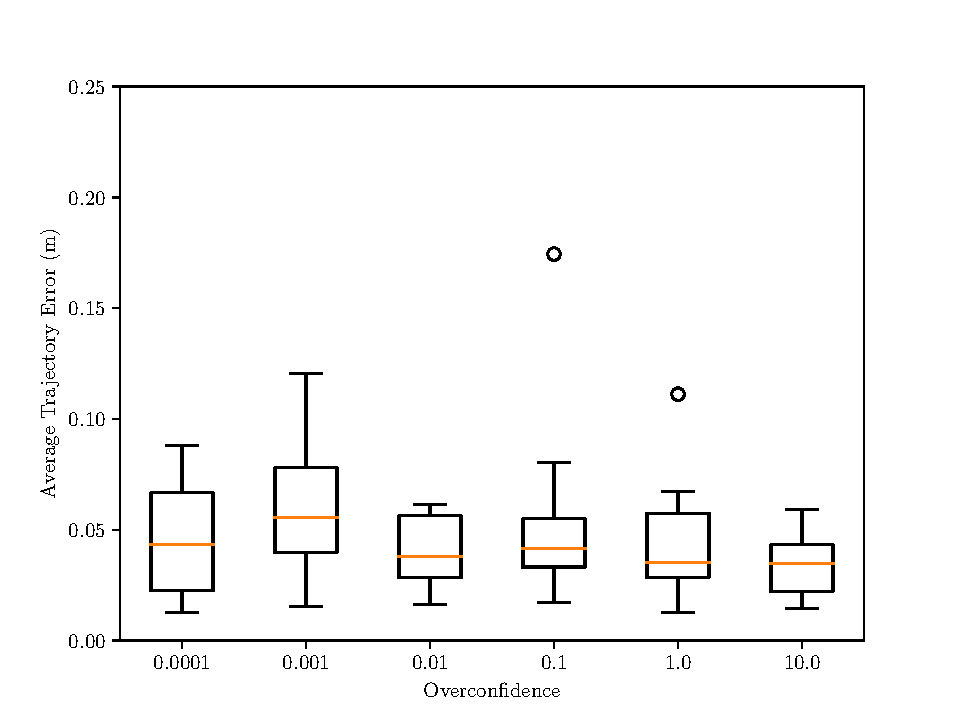
\includegraphics[width=0.45\textwidth]{report/graphs/wartime_overconfidence_resistance_defended.pdf}
		\label{fig:wartime-resistance-defended-overconf}
	}
	\subfigure[Resistance: Without defences]{
		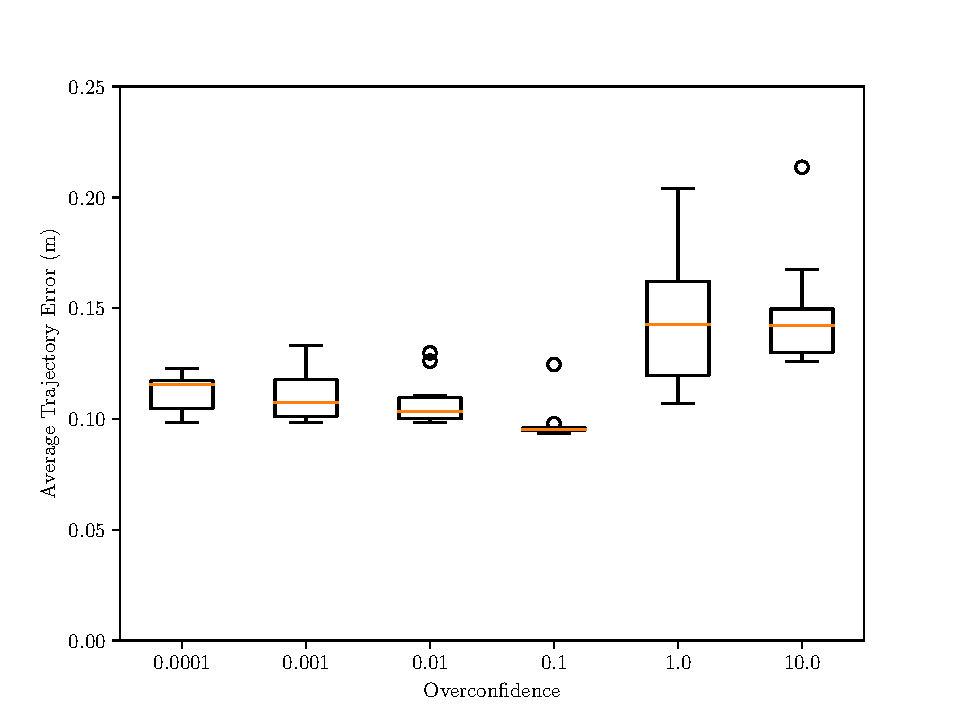
\includegraphics[width=0.45\textwidth]{report/graphs/wartime_overconfidence_resistance_undefended.pdf}
		\label{fig:wartime-resistance-undefended-overconf}
	}
 	\subfigure[Resilience: With defences]{
		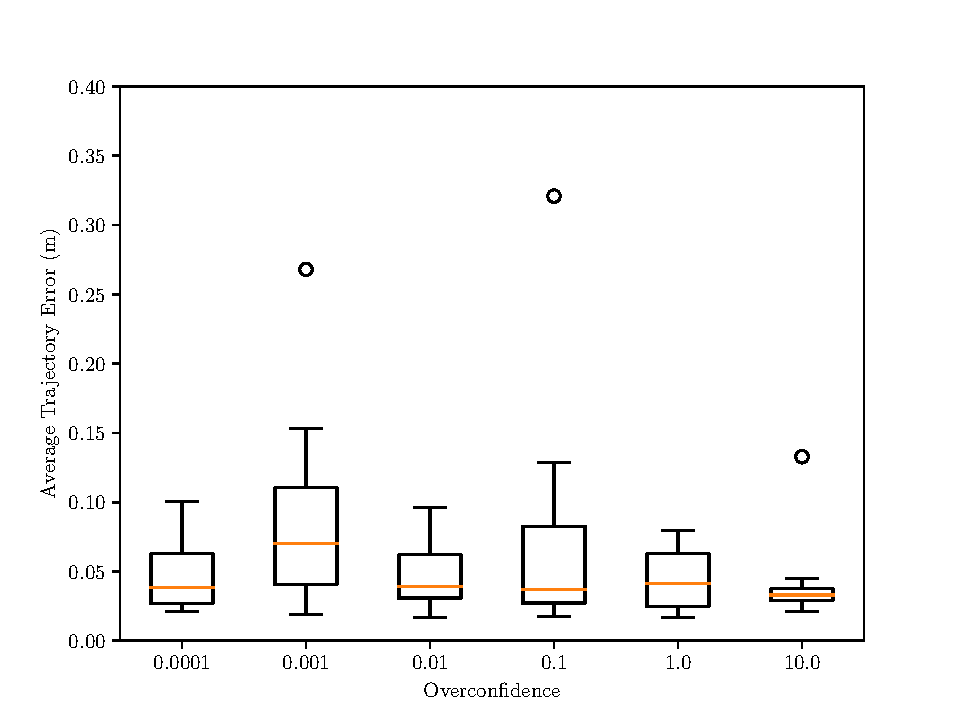
\includegraphics[width=0.45\textwidth]{report/graphs/wartime_overconfidence_resilience_defended.pdf}
		\label{fig:wartime-resilience-defended-overconf}
	}
	\subfigure[Resilience: Without defences]{
		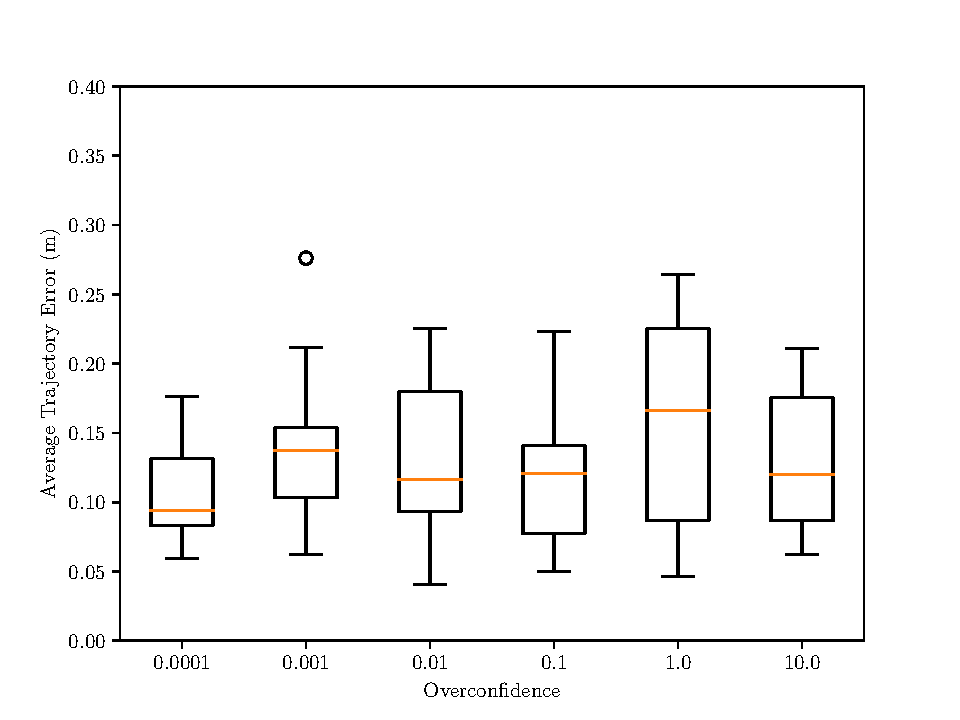
\includegraphics[width=0.45\textwidth]{report/graphs/wartime_overconfidence_resilience_undefended.pdf}
		\label{fig:wartime-resilience-undefended-overconf}
	}
	\caption{Aegis' resistance to and resilience against overconfidence attacks}
        \label{fig:wartime-overconf}
\end{figure}

From \autoref{fig:wartime-overconf}, we make several interesting observations. Firstly, we can see that the resilience of Aegis is worse than its resistance, yet this is likely due to a data imbalance since the group spends less time resisting attacks and more time recovering. We also obtain experimental confirmation that Aegis does successfully protect a group from overconfidence attacks, even as the strength of the attacks increases.

\begin{figure}[!h]
	\centering
	\subfigure[With defences]{
		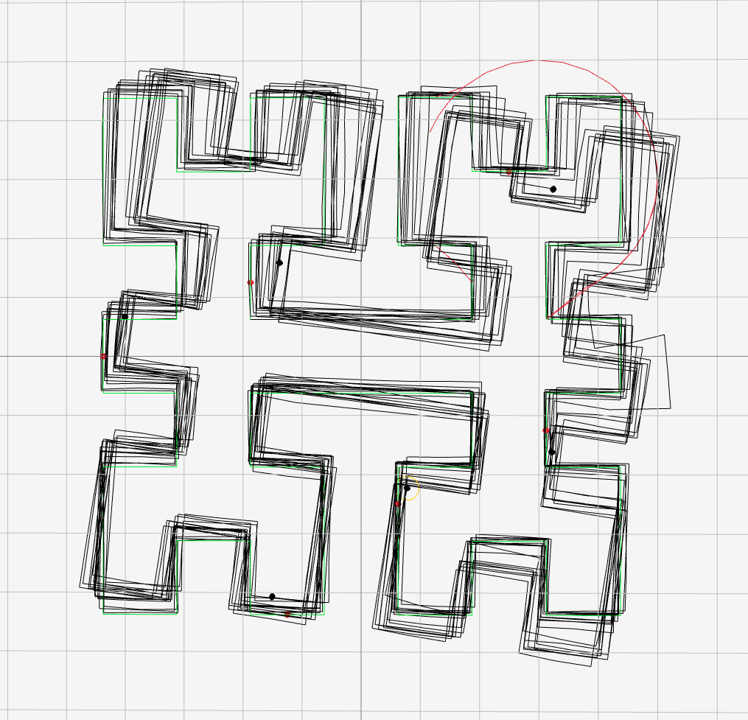
\includegraphics[width=0.45\textwidth]{report/diagrams/defence.png}
	}
	\subfigure[Without defences]{
		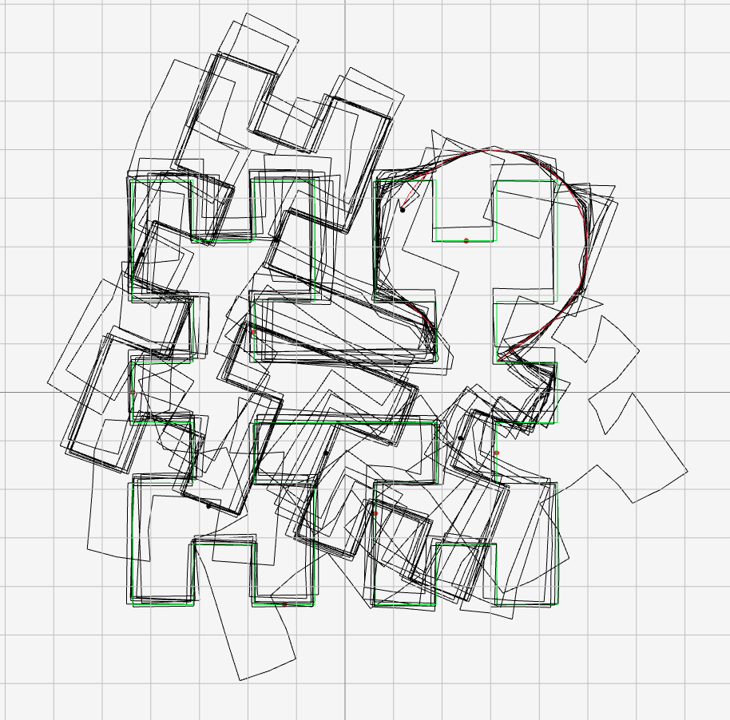
\includegraphics[width=0.45\textwidth]{report/diagrams/undefence.png}
	}
	\caption{Screenshots from the RobotWeb simulator showing the effect of running Aegis. Here the setup is the same as the above experiment and the attacker uses an overconfidence value of 0.01.}
        \label{fig:wartime-overconf}
\end{figure}

\subsubsection{Sybil Attacks should be Ineffective}
Now we repeat the above experiment, but this time using a Sybil attacker. Theoretically, the results of this experiment should match the results of the previous one, however, it is still important to experimentally confirm this. We vary the number of false identities that an attacker can create and measure the group's resistance and resilience. Again we compare this to a scenario without defences, repeating both 10 times. 

\begin{figure}[!h]
	\centering
	\subfigure[Resistance: With defences]{
		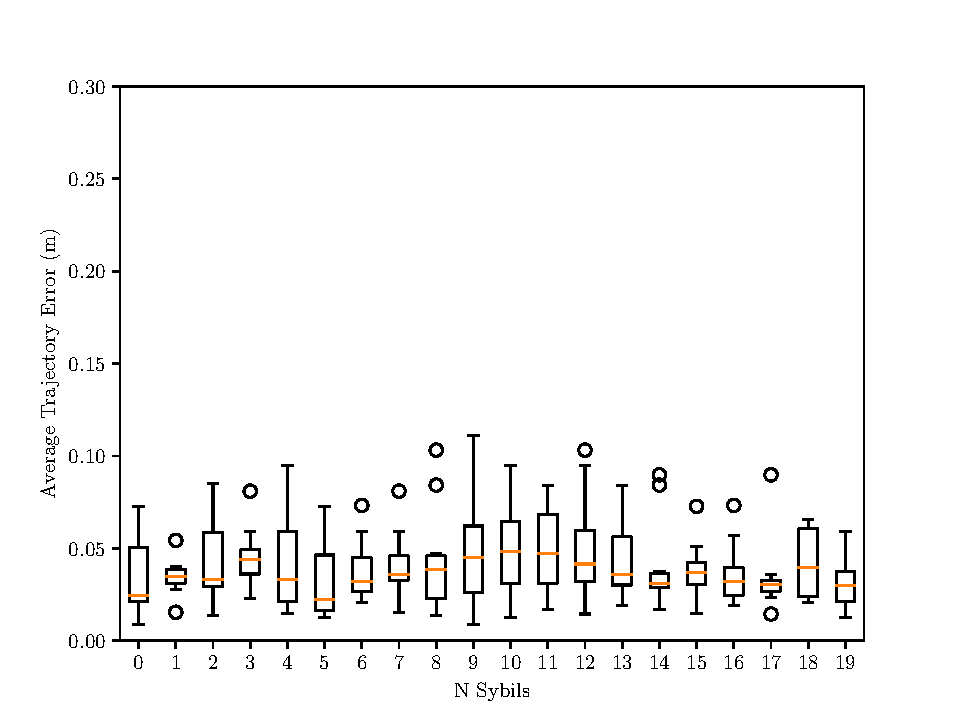
\includegraphics[width=0.45\textwidth]{report/graphs/wartime_sybils_resistance_defended.pdf}
		\label{fig:wartime-defended-resistance-sybil}
	}
	\subfigure[Resistance: Without defences]{
		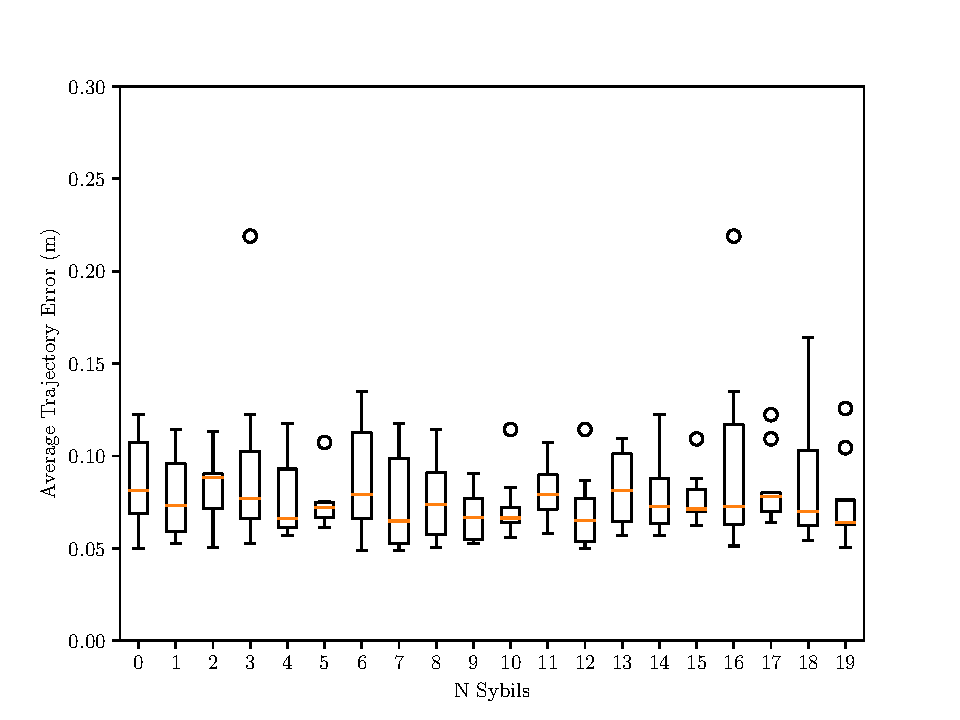
\includegraphics[width=0.45\textwidth]{report/graphs/wartime_sybils_resistance_undefended.pdf}
		\label{fig:wartime-undefended-resistance-sybil}
	}
 	\subfigure[Resilience: With defences]{
		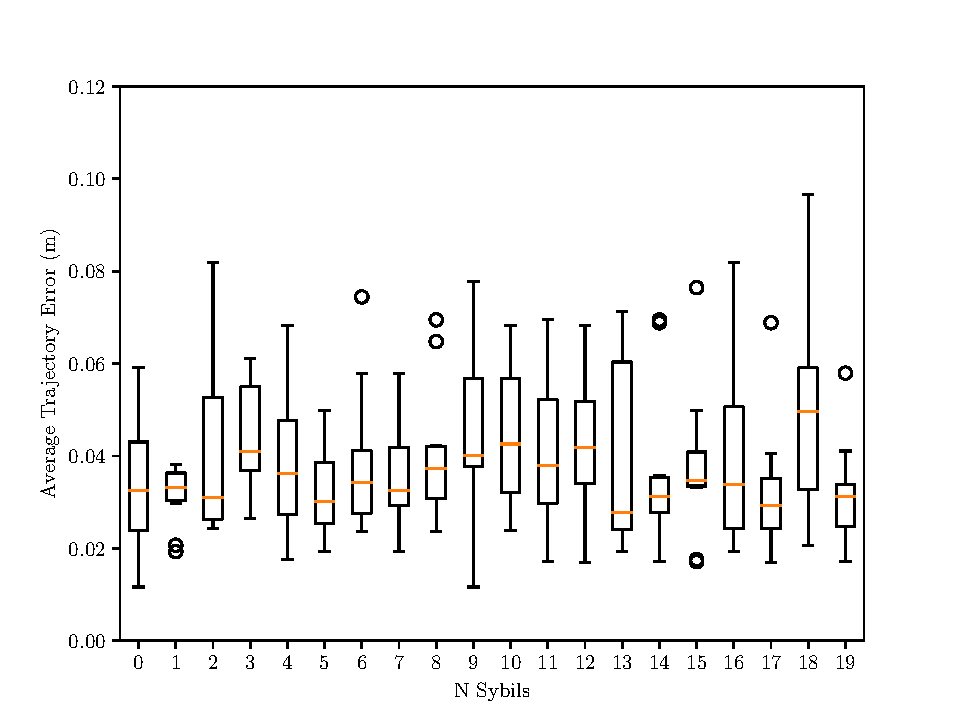
\includegraphics[width=0.45\textwidth]{report/graphs/wartime_sybils_resilience_defended.pdf}
		\label{fig:wartime-defended-resilience-sybil}
	}
	\subfigure[Resilience: Without defences]{
		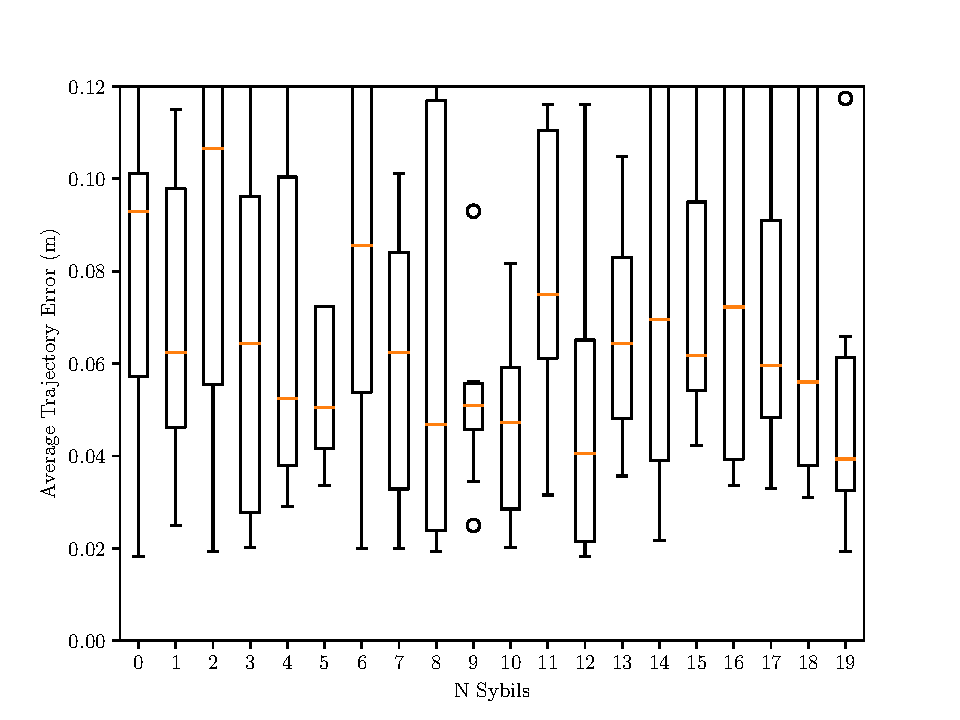
\includegraphics[width=0.45\textwidth]{report/graphs/wartime_sybils_resilience_undefended.pdf}
		\label{fig:wartime-undefended-resilience-sybil}
	}
	\caption{Aegis' resistance to and resilience against Sybil attacks}
         \label{fig:wartime-sybils}
\end{figure}

Again in \autoref{fig:wartime-sybils} we see that the resistance of Aegis is superior to its resilience. We also see that Aegis is resistant against Sybil attacks.

% \subsubsection{Are many groups better than one?}
% Finally, we test whether there is a benefit to using smaller more fragmented groups over larger groups. If there is such a benefit

% We keep the total number of robots constant but vary the number of groups in the simulation. For convenience, we form groups out of adjacent robots. 


% Almost finally, we'll do a bit of a weird one. We'll see how multiple groups interact with one another. We'll keep the total number of robots constant, but vary the number of groups. For convenience, robots near each other on the path will form groups. This might be kinda sus, since we're also changing the group sizes, but if we kept the group size constant, we're also changing the number of robots in total. What we're really getting at though is the relationship between number of robots and the number of groups. Is it better to have more groups or more robots. If it turns out (prolly won't) that more groups is better, then it'll be better for real peeps to have smaller groups. We'll measure perf vs n groups and repeat 10x.

\subsection{Defence when no Attackers are Present}
Now we will evaluate the ATE of Aegis, when no attackers are present. We expect that defended robots will have a slightly higher ATE than undefended robots. The reason behind this is that undefended robots are able to participate more than defended robots since they \begin{enumerate*}
    \item do not reject any messages and
    \item have no leaders which are isolated from the RobotWeb
\end{enumerate*}, which should allow them to reap more of the benefits of participation.

We measure the cost of defence by running the simulation both with and without defences, repeating this 10 times.
\begin{figure}[!h]
	\centering
        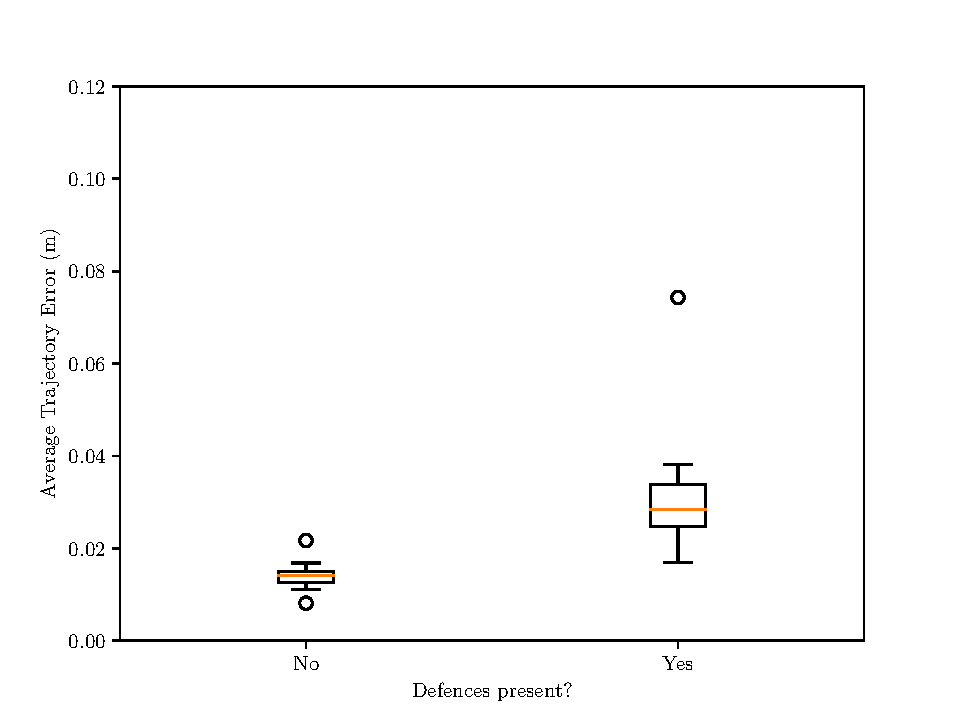
\includegraphics[width=7cm]{report/graphs/peacetime.pdf}
	\caption{The cost of using defences when no attackers are present.}
        \label{fig:peacetime}
\end{figure}

Now from \autoref{fig:peacetime}, we can see that running Aegis does incur a performance penalty when no attackers are present. In fact, we can see that the addition of Aegis, almost doubles the ATE of robots. This is in line with our expectations as defended robots participate less in the RobotWeb, and so reap fewer of its benefits. Here no leader has any compatriots, and so they are essentially isolated, increasing their ATE, whilst their followers rely upon these worsened messages.

However, the decrease in performance is still quite small in absolute terms as it translates to an additional 0.015m of ATE. It is for this reason that we do not believe that the cost of Aegis is prohibitive to its usage.

Most importantly, if we compare these results to \autoref{fig:wartime-overconf} and \autoref{fig:wartime-sybils}, we see that the ATE when attackers are present is the same as when attackers are absent, once more experimentally confirming the potency of Aegis.

\subsubsection{Measuring the Effect of Multiple Groups}
In the above experiments, we only considered a single group, however in a real-world setting Aegis is likely to run on multiple groups, which mutually distrust one another. We will now briefly consider the effect including multiple groups, and varying their sizes, will have upon the performance of Aegis.

We will vary the size of the groups from 1 to 4, and also vary the number of groups from 1 to 4.
\begin{figure}[!h]
	\centering
	\subfigure[Resistance]{
		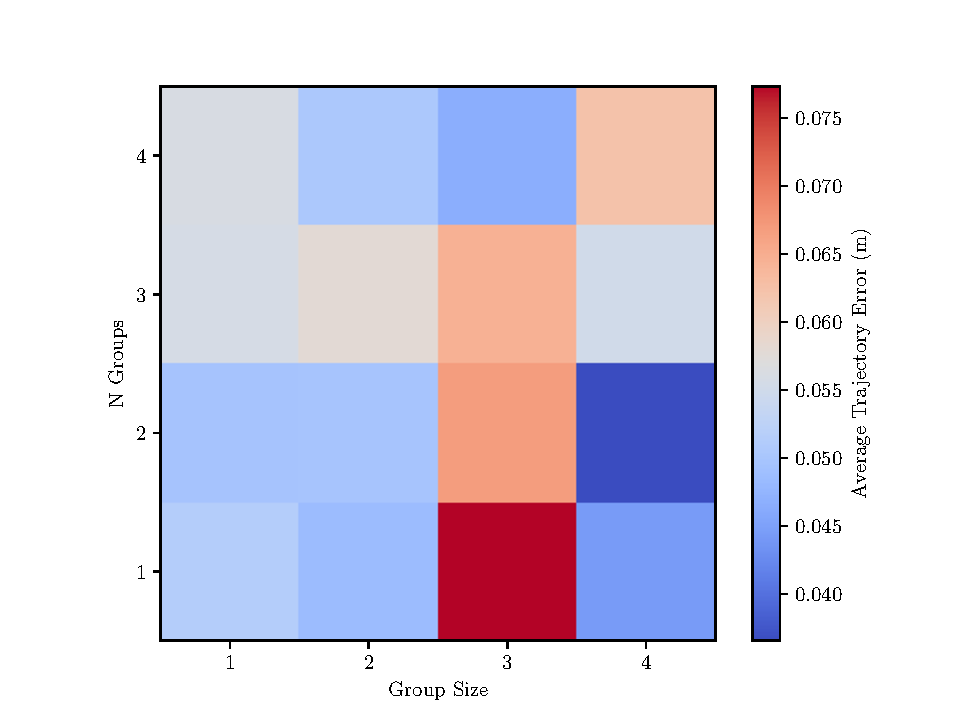
\includegraphics[width=0.3\textwidth]{report/graphs/n_groups_resistance.pdf}
		\label{fig:n-groups-resistance}
	}
	\subfigure[Resilience]{
		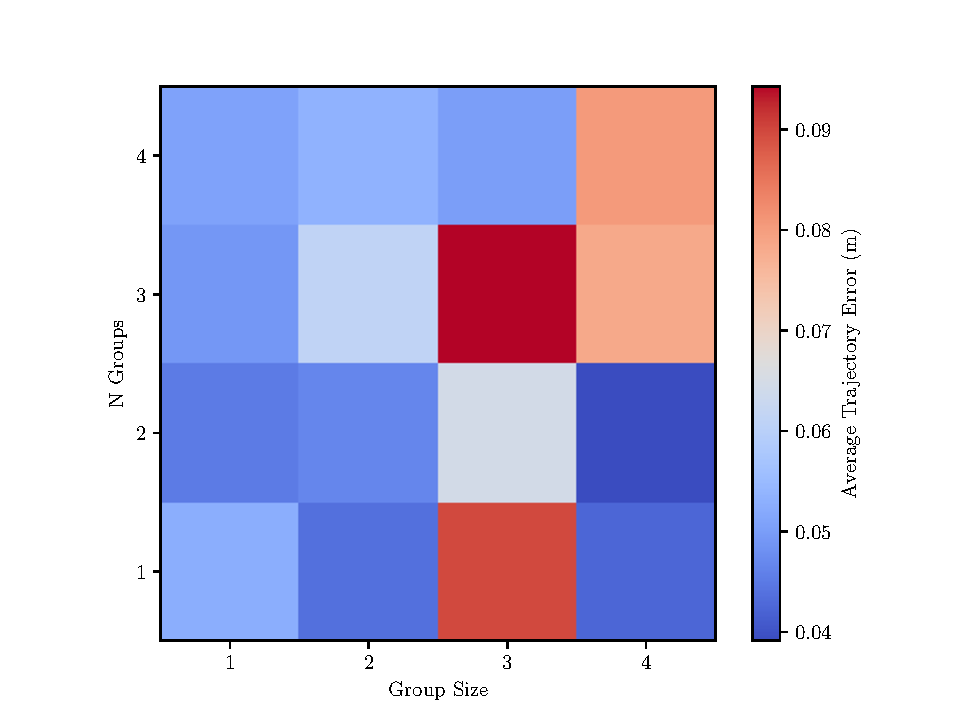
\includegraphics[width=0.3\textwidth]{report/graphs/n_groups_resilience.pdf}
		\label{fig:n-groups-resilience}
	}
 	\subfigure[Cost of Operation]{
		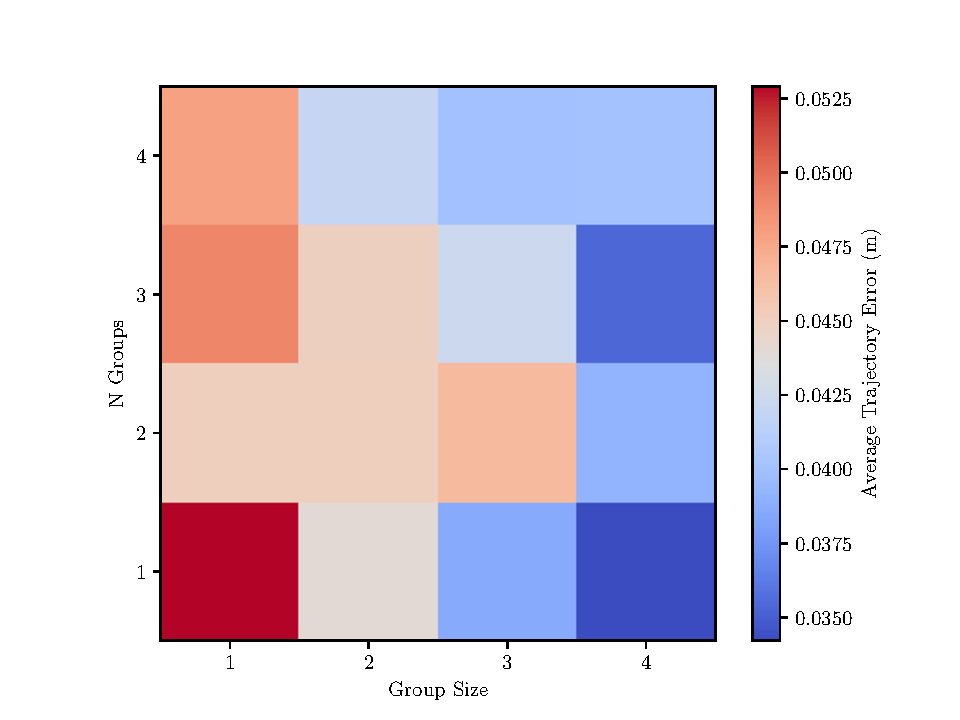
\includegraphics[width=0.3\textwidth]{report/graphs/n_groups_reduction.pdf}
		\label{fig:n-groups-reduction}
	}
	\caption{Varying the number of groups and the overall group sizes.}
\end{figure}

Examining \autoref{fig:n-groups-resistance} and \autoref{fig:n-groups-resilience}, we see no pattern in the performance, but we do see a markedly worse performance when the group size is 3, however, we do not believe that this effect is inherent to Aegis, instead it is likely to be a combination of the quirks of the environment and particular set of parameters used in this experiment. Now looking at the cost of operation, \autoref{fig:n-groups-reduction}, we see that increasing the number of groups does lead to a marked increase in the overall performance, as does increasing the group size. Furthermore, looking at the diagonals, we can see that increasing the size of a group leads to a lower cost than increasing the number of groups, which is likely due to the fact that robots inside a group have the guarantee of mutual trust, and so do not tend to reject one another's messages.

\subsection{Tuning the Parameters of Aegis} \label{section:optim}
In the previous sections, we used random policies and an arbitrary set of parameters to evaluate Aegis, yet these are unlikely to produce the best performance. Firstly, it is likely that a more carefully crafted Successor Identification or Retirement Policy would outperform a random policy. Secondly, it is also likely that varying both the minimum and maximum number of leaders in a group would have an effect on performance. Finally, it is also likely that the \textit{leader divergence} - $\epsilon$, plays a significant role in the final performance outcome.

We will now test these claims by comparing the performances of several alternative policies as well as by varying the aforementioned parameters. We will evaluate these when the group is both under attack and safe, in order to gain a holistic understanding of its strength, and costs.

A challenge that arises here, is that it is difficult to judge the relative weightings between these two situations. Firstly, because we have no data to indicate how often a robot should expect to be attacked. Secondly, we also cannot reliably estimate how harmful an attack would be, since this varies across use cases. We resolve this problem by not resolving it - we will instead compare the resistance, resilience and cost of operation, separately. We believe that this allows for a deeper understanding of the performance characteristics of our defence than a single value would, and thus be of greater decision-making value.

\subsubsection{Comparing different Retirement Policies}
We compare the random retirement policy with two new ones - a Fixed-Term Retirement Policy (FTRP) and a Confidence-Based Retirement Policy (CBRP). All three of these policies have their own configurable parameters, hence we must find their optimal parameters before we can compare them with one another.

In a random retirement policy, a leader can resign at any tick, with probability $p$. To find the best possible random retirement policy, we must find the optimal value of $p$. We do this by varying $p$ from 0.1 to 1, in increments of 0.1.
\begin{figure}[!h]
	\centering
	\subfigure[Resistance]{
		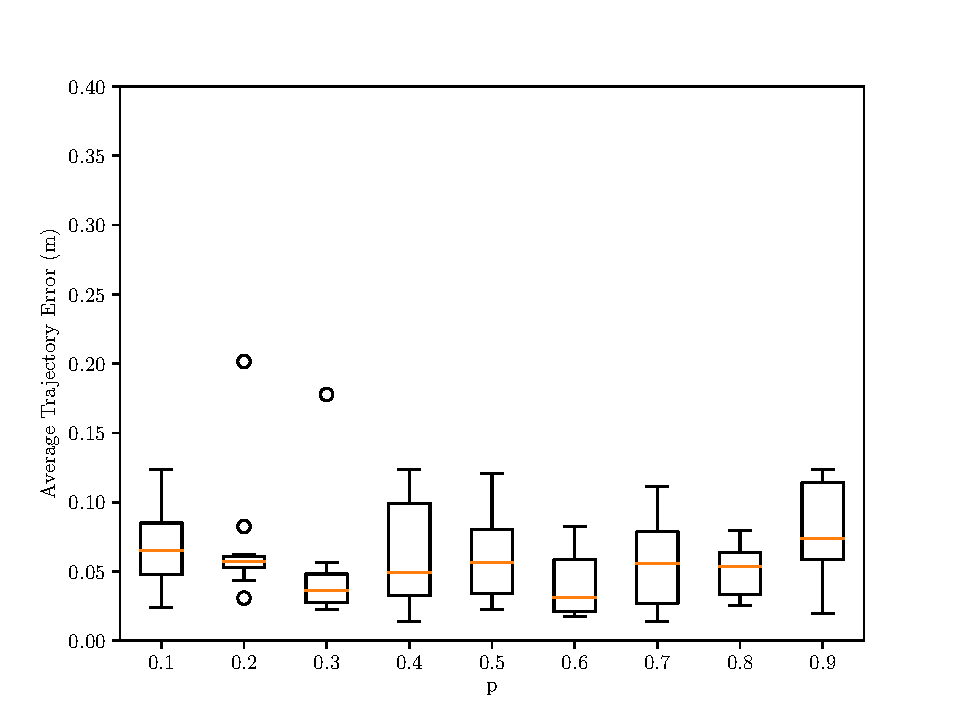
\includegraphics[width=0.3\textwidth]{report/graphs/random_resistance.pdf}
		\label{fig:random-resistance}
	}
	\subfigure[Resilience]{
		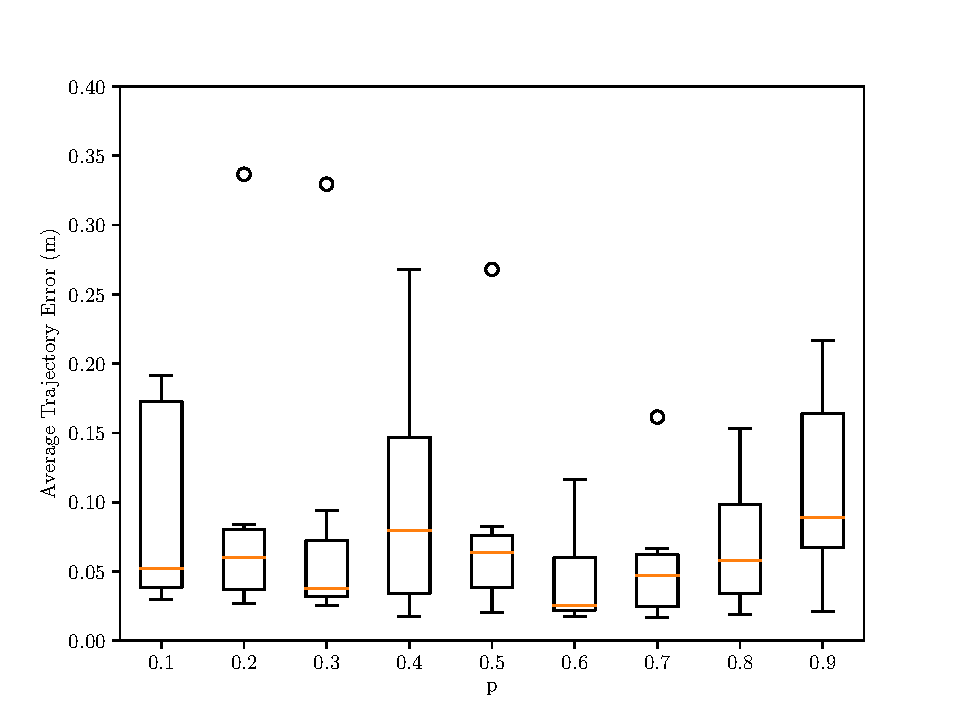
\includegraphics[width=0.3\textwidth]{report/graphs/random_resilience.pdf}
		\label{fig:random-resilience}
	}
 	\subfigure[Cost of Operation]{
		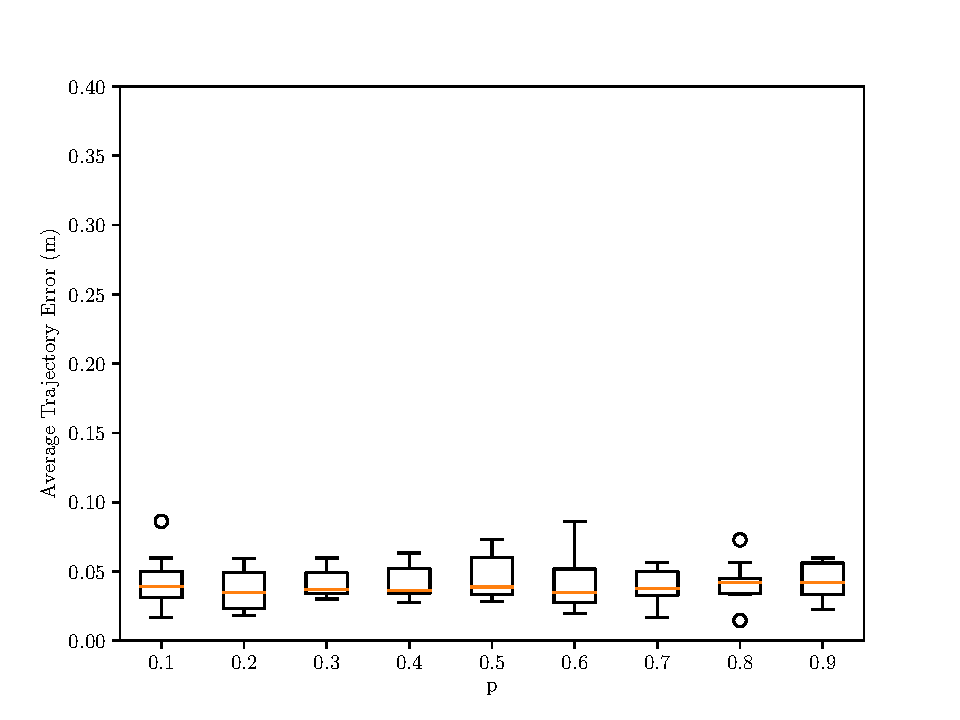
\includegraphics[width=0.3\textwidth]{report/graphs/random_reduction.pdf}
		\label{fig:random-reduction}
	}
	\caption{Finding the optimal value of $p$ for a random retirement policy}
        \label{fig:random}
\end{figure}

Looking at \label{fig:random}, we see no correlation between the probability of retirement, $p$, and the overall performance of Aegis. However, we do see a slight preference towards $p = 0.5$, when looking at the resilience, \autoref{fig:random-resilience}, which translates to an expected term length of 2. Yet we do not observe the same effect when using a FTRP in \autoref{fig:fixed-resilience}. This leads us to suspect that either all random policies are equal, or that more comprehensive experimentation is needed to truly measure its effect.

In a FTRP, leaders will retire after serving for a fixed, term length, $t$. We now vary the value of $t$ between 1 and 20 to observe the effect of the term length on the performance of Aegis. We will repeat each experiment 10 times.

\begin{figure}[!h]
	\centering
	\subfigure[Resistance]{
		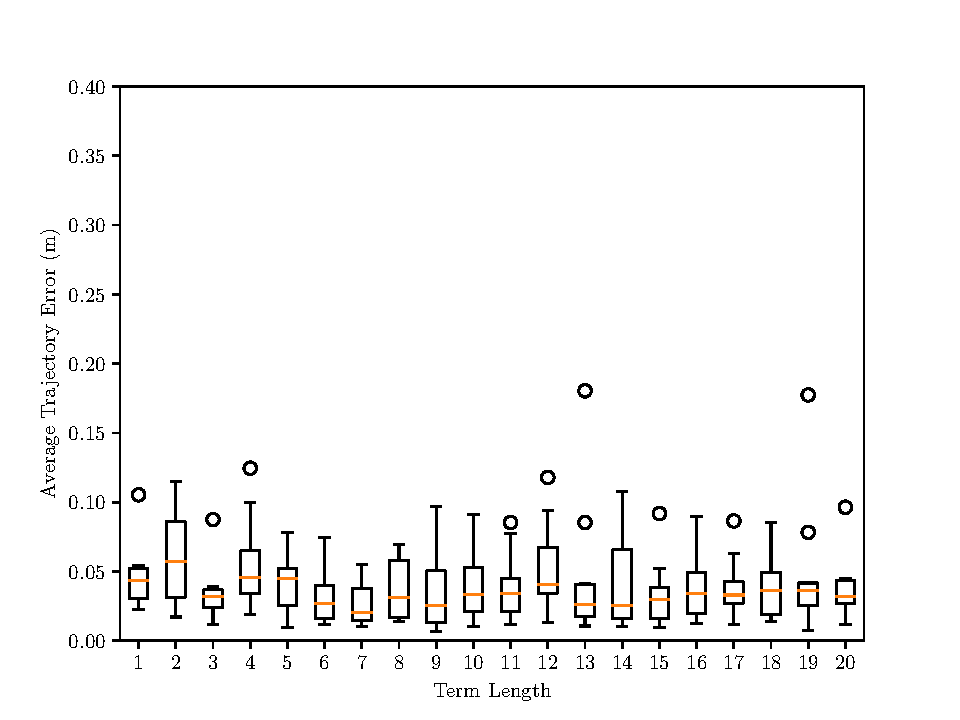
\includegraphics[width=0.3\textwidth]{report/graphs/fixed_term_resistance.pdf}
		\label{fig:fixed-resistance}
	}
	\subfigure[Resilience]{
		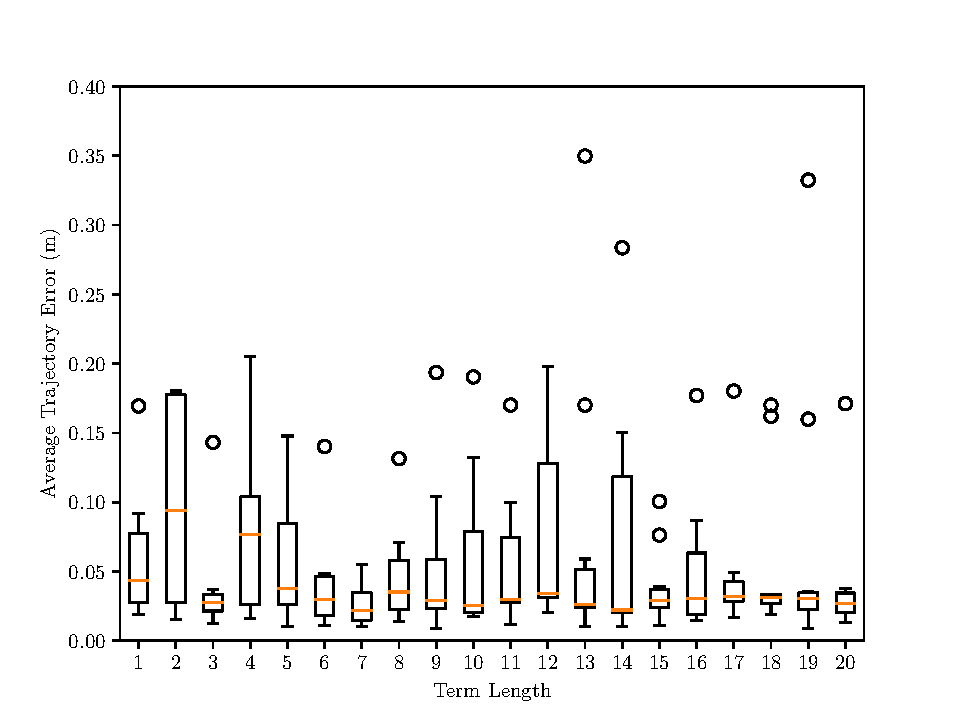
\includegraphics[width=0.3\textwidth]{report/graphs/fixed_term_resilience.pdf}
		\label{fig:fixed-resilience}
	}
 	\subfigure[Cost of Operation]{
		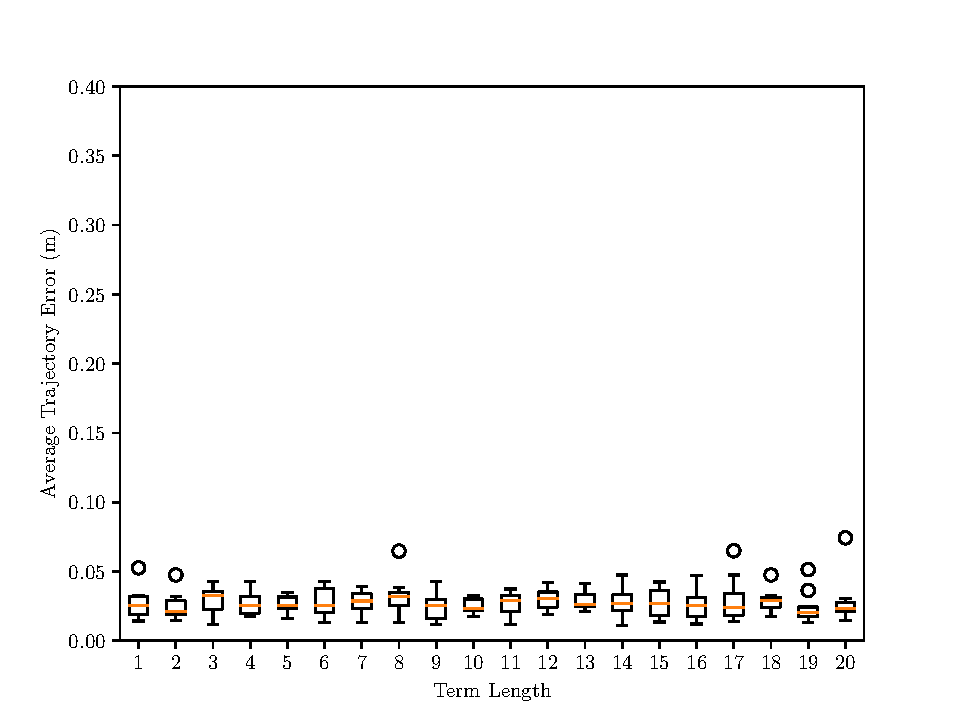
\includegraphics[width=0.3\textwidth]{report/graphs/fixed_term_reduction.pdf}
		\label{fig:fixed-reduction}
	}
	\caption{Finding the optimal length for a FTRP}
        \label{fig:fixed}
\end{figure}

Looking at \autoref{fig:fixed}, we find no correlation between the length of a term and the overall performance of the FTRP. However, this defies our earlier theory, that longer term lengths should result in worse performances. We again suspect that further investigation is required to verify this.

A CBRP is more complex, here a leader will only retire if its confidence in its localisation falls below the threshold $c$. This aims to ensure that leaders will serve for as long as possible before retiring. However, this ``confidence'' value is hard to define, as a robot's confidence is represented by the values in its precision matrix, $\Lambda$, which contains more than 1 value. So to implement CBRP, we must first define the ``confidence'' of a robot. We define it as the smallest eigenvalue of $\Lambda$. We now vary $c$ from 0.0001 to 10, and repeat each experiment 10 times.

\begin{figure}[!h]
	\centering
	\subfigure[Resistance]{
		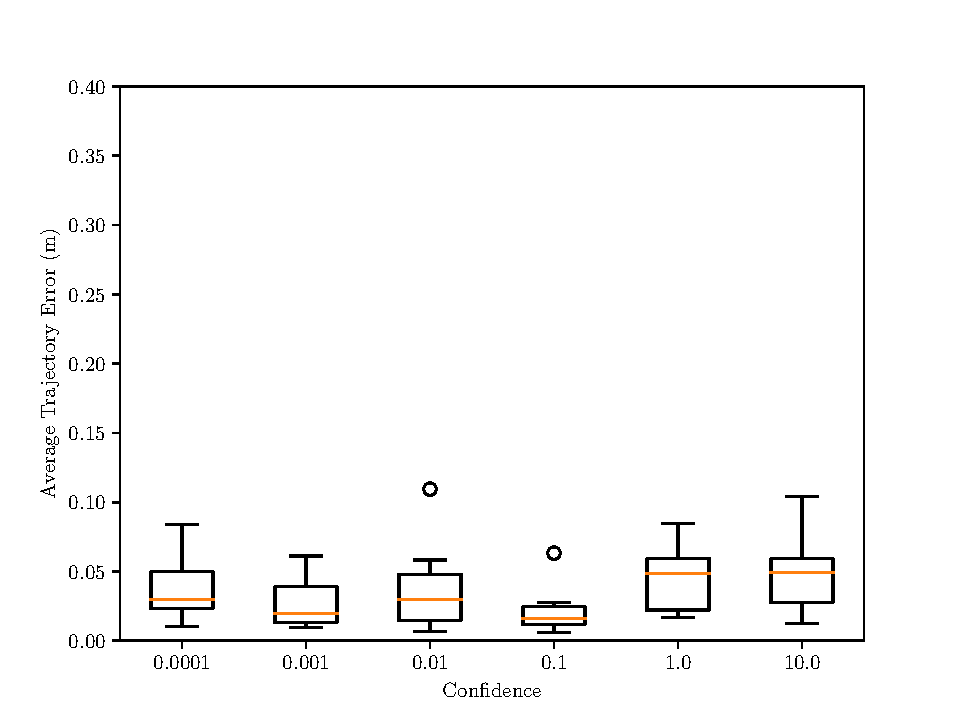
\includegraphics[width=0.3\textwidth]{report/graphs/confidence_based_resistance.pdf}
		\label{fig:conf-resistance}
	}
	\subfigure[Resilience]{
		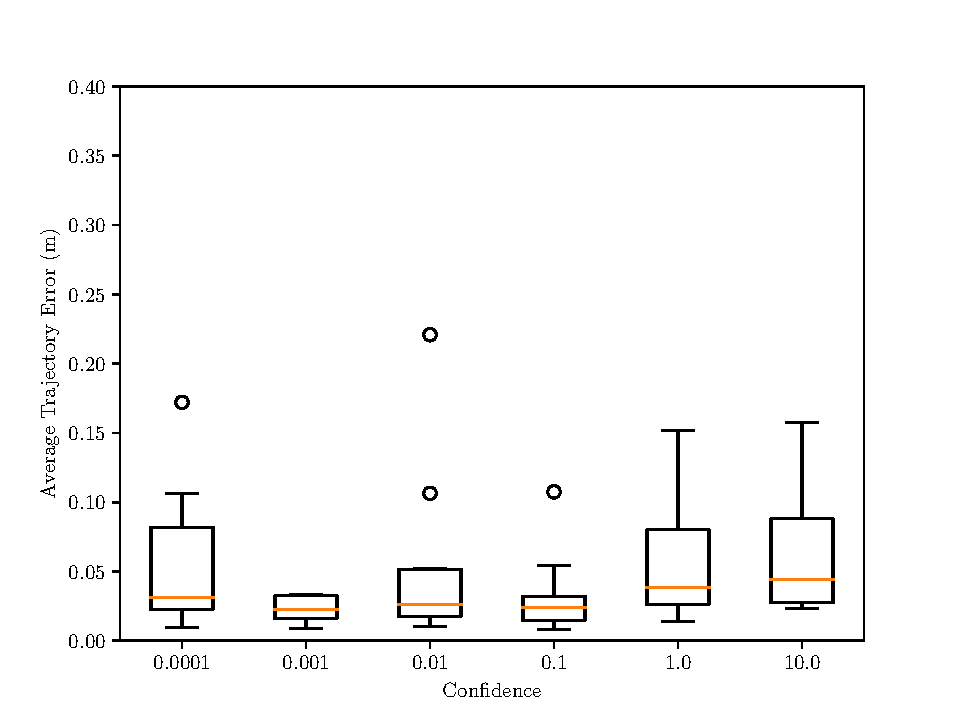
\includegraphics[width=0.3\textwidth]{report/graphs/confidence_based_resilience.pdf}
		\label{fig:conf-resilience}
	}
 	\subfigure[Cost of Operation]{
		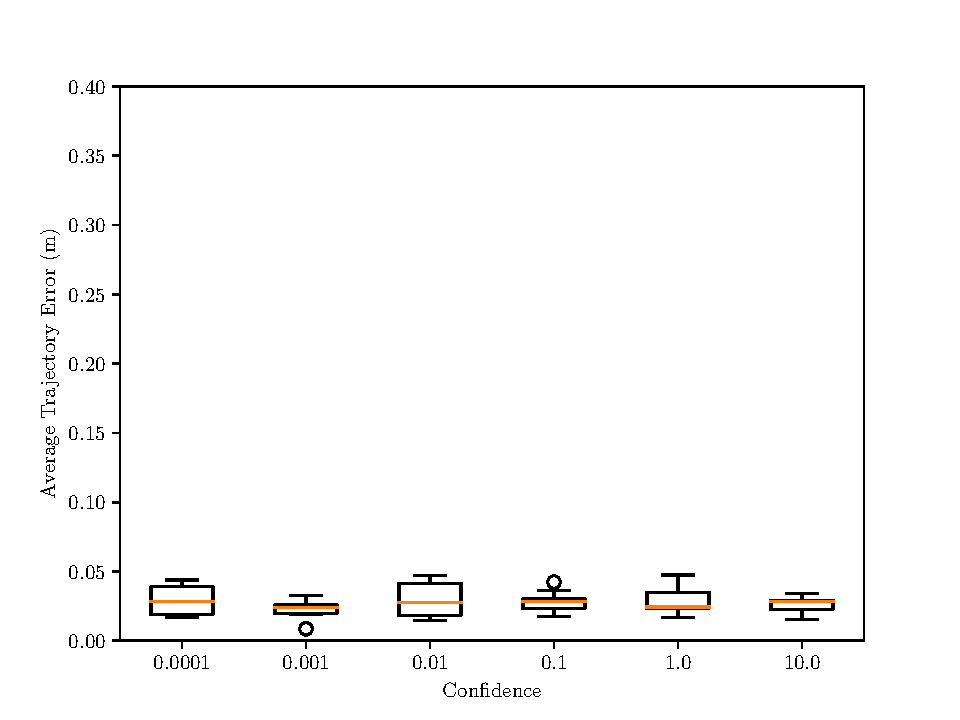
\includegraphics[width=0.3\textwidth]{report/graphs/confidence_based_reduction.pdf}
		\label{fig:conf-reduction}
	}
	\caption{Finding the optimal confidence threshold for a CBRP}
        \label{fig:conf}
\end{figure}

From \autoref{fig:conf}, we can see that the confidence threshold does not have an impact on the resistance, resilience, or cost of operation of Aegis. However, we also see a noticeable improvement in performance across all metrics, which indicates that a CBRP is a more suitable choice. These results also lead us to suspect that the reason why the previous experiments showed no correlation between the length of a leader's term and performance, is because there truly is no correlation between them. However, this remains to be confirmed.

In conclusion, we believe that a CBRP is the best choice of policy and that future work in improving Aegis' policies should use it as a starting point, rather than using any time based retirement policies.

\subsubsection{Comparing different Successor Identification Policies}
We now compare the random successor identification policy with three new ones - a Least-Recently-Lead (LRL-SIP), a Confidence-Based (CB-SIP), and a Centroid (C-SIP) successor identification policy. Neither of these has any configurable parameters, allowing us to directly compare them without first tuning either.

A LRL-SIP aims to promote fairness, where each robot has an equal opportunity to become a leader. Here a leader will choose the follower who led the longest time ago. This ensures that no robot spends too much time as a follower. However, it makes its decision whilst eschewing the suitability of each potential successor. For example, a robot with lower confidence could be chosen over one with higher confidence, which should prove detrimental to the quality of the entire group's localisations.

A CB-SIP aims to remedy this, by choosing the robot with the highest confidence. Once again, the confidence of a robot is defined as the smallest eigenvalue of its precision matrix, $\Lambda$. However, this approach has a glaring fault - it can allow attackers to gain influence. Since followers are weakly-defended, their confidences can be artificially increased. Now an attacker may ensure that certain robots are chosen, by increasing their confidences. And since attackers are hostile, these are likely to be poor choices. However, the feasibility of this as an attack vector is debatable, as attackers would need to know which robots are leaders and which are followers.

Finally, a C-SIP aims to choose leaders who will serve the most number of robots. A leader following a C-SIP will find the centroid of its known followers, and then choose the follower closest to that centroid. This should ensure that the chosen robot serves as many followers as possible. 

We now compare the performance of each SIP, repeating each experiment 10 times.

\begin{figure}[!h]
	\centering
	\subfigure[Resistance]{
		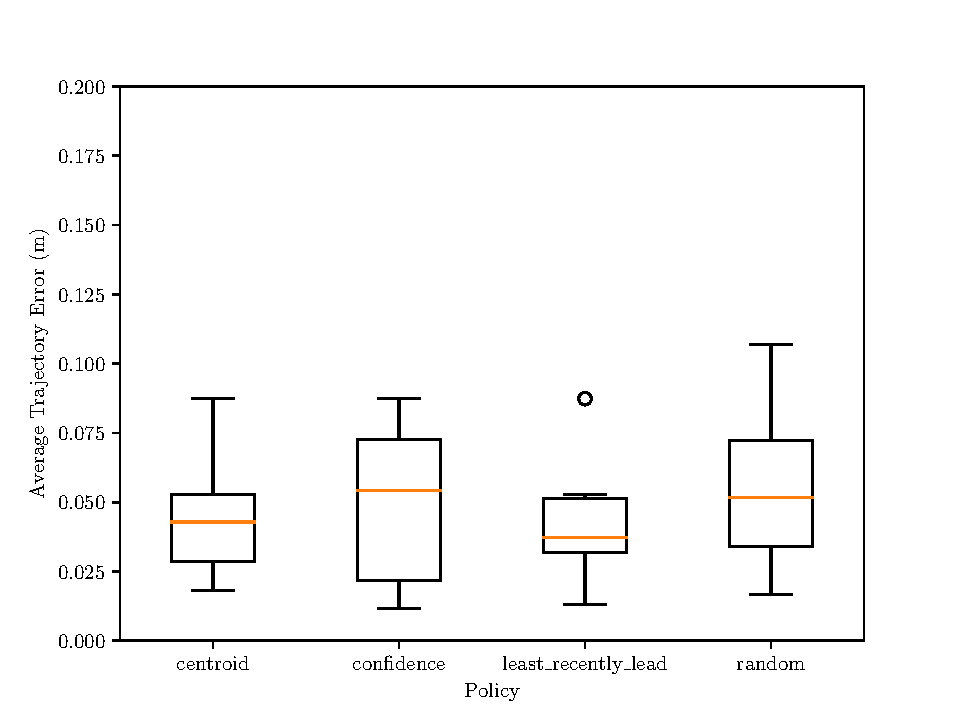
\includegraphics[width=0.3\textwidth]{report/graphs/policy_resistance.pdf}
		\label{fig:policy-resistance}
	}
	\subfigure[Resilience]{
		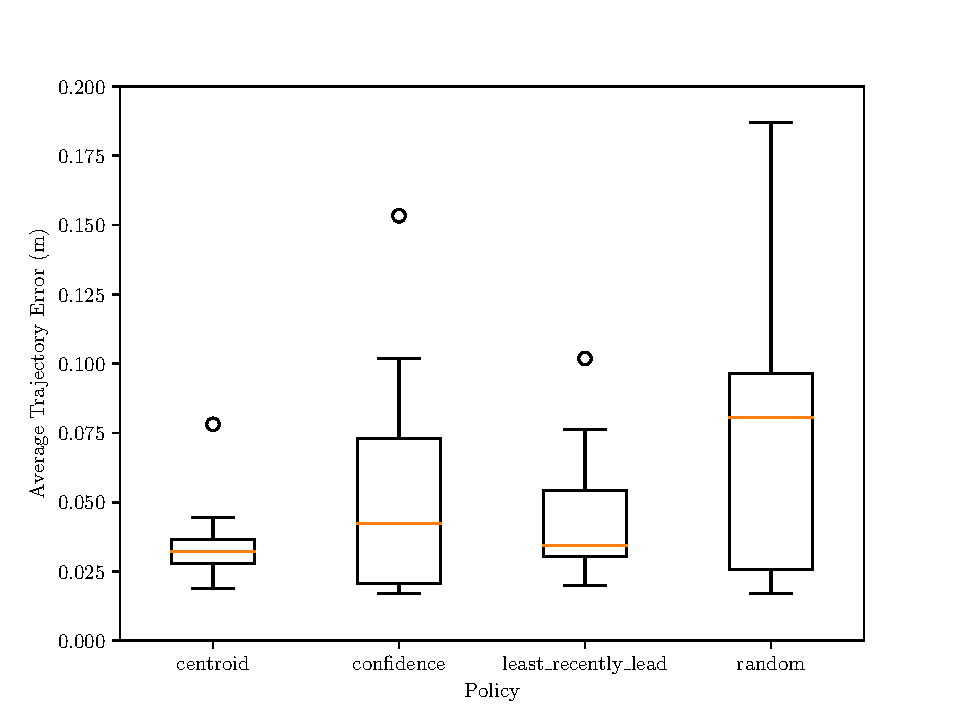
\includegraphics[width=0.3\textwidth]{report/graphs/policy_resilience.pdf}
		\label{fig:policy-resilience}
	}
 	\subfigure[Cost of Operation]{
		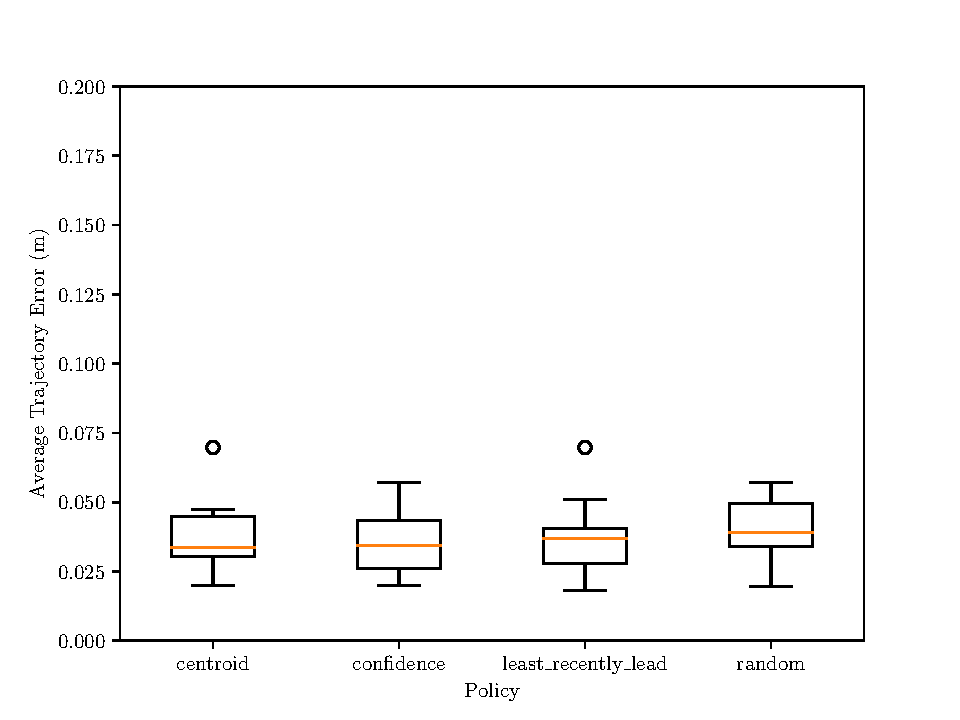
\includegraphics[width=0.3\textwidth]{report/graphs/policy_reduction.pdf}
		\label{fig:policy-reduction}
	}
	\caption{Comparing between a Random, Least-Recently-Lead, Confidence-Based, and Centroid Successor Identification Policy}
        \label{fig:policy}
\end{figure}

Looking at \autoref{fig:policy-resistance}, we see that all four policies have comparable performances when it comes to their ability to resist attacks, yet when we examine \autoref{fig:policy-resilience}, we see that the C-SIP decisively outperforms the others. This effect may be due to the fact that the baseline estimates formed using a central (not centralised) leader are simply more confident than those formed by others. This would occur as the quality of a leader's measurements, decreases as the follower it is measuring moves further from it. Finally looking at the Cost of Operation in \autoref{fig:policy-reduction}, we again see no clear difference between successor identification policies.

\subsubsection{Varying the Permissiveness of Followers}
The permissiveness of a follower refers to how far a message can be from the baseline estimate for it to still be accepted. This variable is represented by the $\epsilon$ (the \textbf{Maximum Leader Divergence}) parameter. We believe that a follower's permissiveness should occupy a ``Goldilocks Zone'' being neither too high nor too low. If a follower is too permissive, then it can be easily exploited by attackers, who would have a large range of localisations to force it to. On the other hand, a follower that is too strict would ignore many helpful messages. This leads us to believe that an optimal level of permissiveness exists.

\begin{figure}
    \centering
    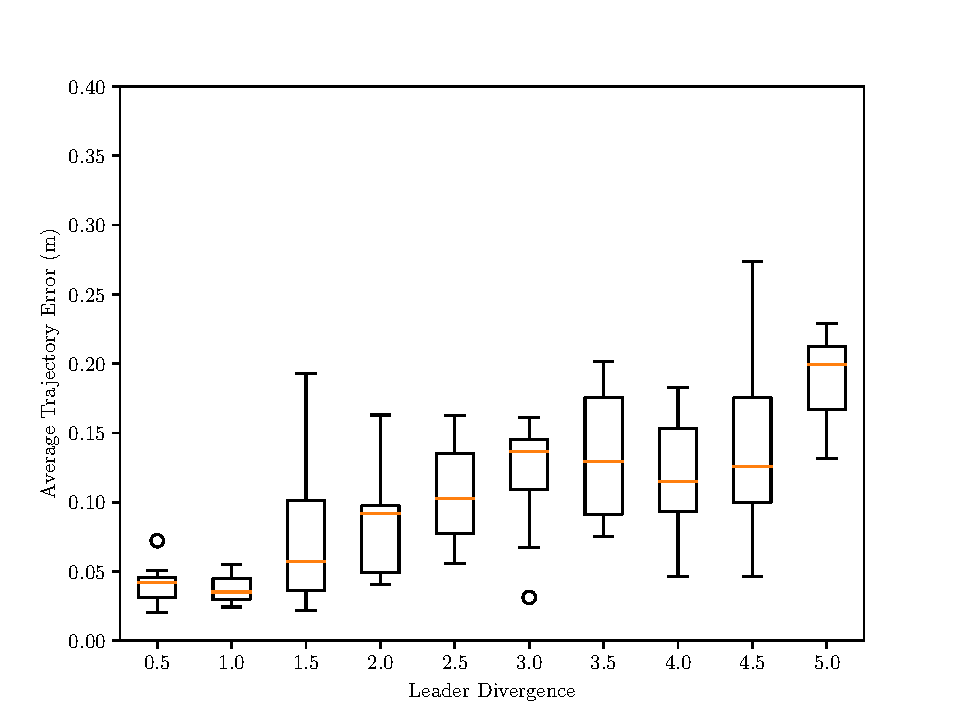
\includegraphics[width=7cm]{report/graphs/leader_divergence_max.pdf}
    \caption{Finding the optimal value $\epsilon$ for the permissiveness of a follower}
    \label{fig:leader-div}
\end{figure}

In \autoref{fig:leader-div} we see a clear trend confirming our hypothesis, as increasing the divergence of a leader subsequently decreases its performance. We also see this effect plateau when $\epsilon$ falls below 1. This plateau is likely caused by the followers only listening to their leaders, rather than one another. In fact, we believe that if this experiment were to be rerun with many robots and many groups, then the effect of this plateau would be more pronounced, as robots further lose their ability to benefit from others.

\subsubsection{Varying the Number of Leaders}
The final parameters we tune are the minimum and maximum numbers of leaders respectfully. We believe that increasing the minimum number of leaders will have a more pronounced effect than increasing the maximum number of leaders. The reason for this is that there \textit{must} be at least $L_{min}$ leaders, but there \textit{can} be upto $L_{max}$ leaders, so increasing $L_{max}$ does not necessarily increase the actual number of leaders in a group. Nevertheless, we believe that increasing the number of leaders will improve the resistance and resilience of a group, whilst simultaneously worsening the cost of operating Aegis.

We now vary $L_{min}$ and $L_{max}$ from 1 to 4, repeating each experiment 10 times.
\begin{figure}[!ht]
	\centering
	\subfigure[Resistance]{
		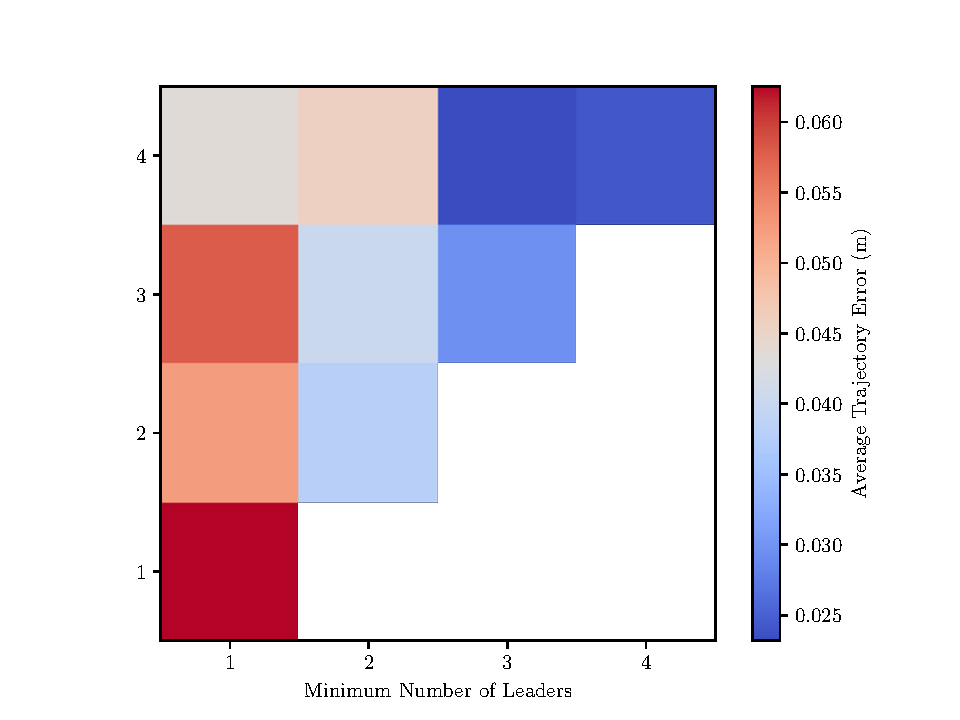
\includegraphics[width=0.3\textwidth]{report/graphs/n_leaders_resistance.pdf}
		\label{fig:n-leaders-resistance}
	}
	\subfigure[Resilience]{
		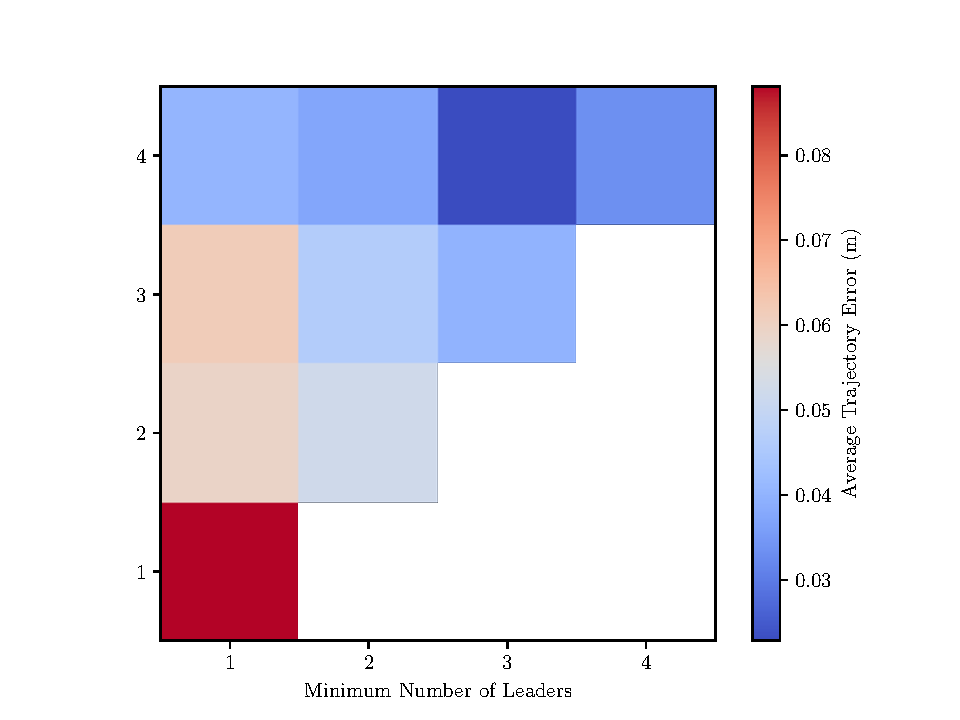
\includegraphics[width=0.3\textwidth]{report/graphs/n_leaders_resilience.pdf}
		\label{fig:n-leaders-resilience}
	}
 	\subfigure[Cost of Operation]{
		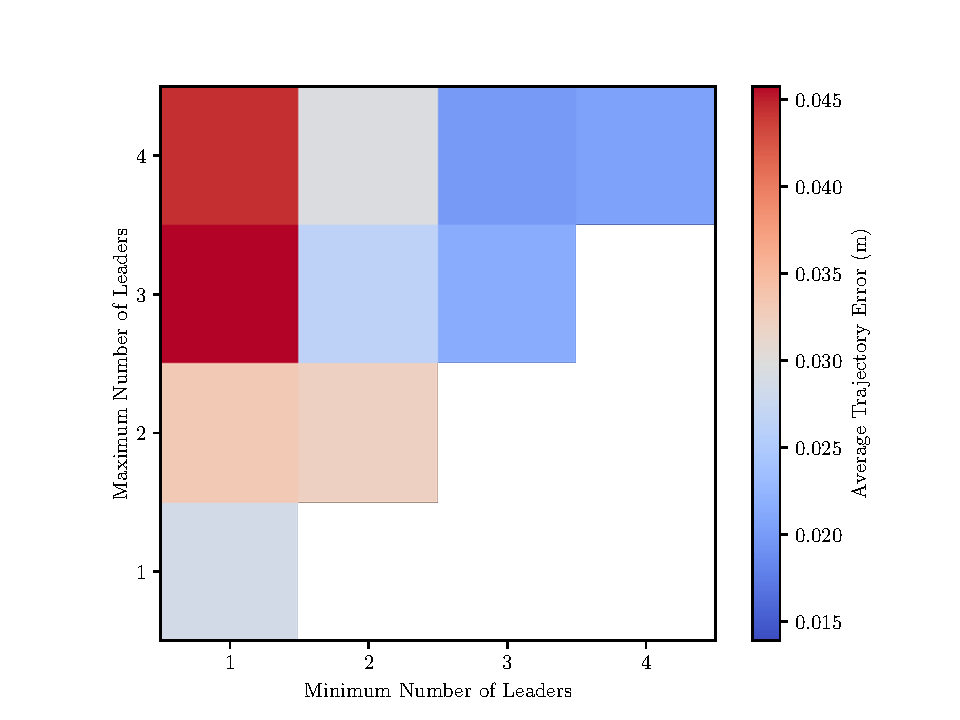
\includegraphics[width=0.3\textwidth]{report/graphs/n_leaders_reduction.pdf}
		\label{fig:n-leaders-reduction}
	}
	\caption{Varying $L_{min}$ and $L_{max}$}
\end{figure}

From \autoref{fig:n-leaders-resistance} and \autoref{fig:n-leaders-resilience}, we can see a marked improvement in performance as both $L_{min}$ and $L_{max}$ increase, notably an increase in $L_{min}$ affects the performance more than one in $L_{max}$, confirming our theory. We also see in \autoref{fig:n-leaders-reduction}, that increasing $L_{max}$ does increase the cost of operation, yet increasing $L_{min}$ does not.